\makeatletter
\def\input@path{{../}}
\makeatother
\documentclass[../main.tex]{subfiles}
\begin{document}
\renewcommand{\path}{3_chapter_1/}
\chapter[RestraintMaker: A Graph-Based Approach to Select Distance Restraints in Free-Energy Calculations with Dual Topology]{RestraintMaker: A Graph-Based Approach to Select Distance Restraints in Free-Energy Calculations with Dual Topology
    \footnote{\label{footnoteChapter2CopyRight} 
    This Chapter is reproduced in part from  Benjamin Ries$^\dag$, Salom\'e Rieder$^\dag$, Clemens Rhiner, Philippe H. H\"unenberger, and Sereina Riniker,
 J. Comput.-Aided Mol. Des., submitted (2021). $^\dag$ These authors contributed equally.}
 }
\chaptermark{RestraintMaker}
\label{ch:feres}

\aquote{
    "Allzu straff gespannt, zerspringt der Bogen."\\ \color{OliveGreen} \footnotesize{``And much too tightly stretched the bow will split.''}
}{Rudenz in Wilhelm Tell\\ Friedrich Schiller\cite{Schiller1898}}



\begin{summary}
The calculation of relative binding free energies (RBFE) involves the choice of the end-state/system representation, of a sampling approach, and of a free-energy estimator. System representations are usually termed ``single topology'' or ``dual topology''. As the terminology is often used ambiguously in the literature, a systematic categorization of the system representations is suggested here. In the dual topology approach, the molecules are simulated as separate molecules. Such an approach is relatively easy to automate for high-throughput RBFE calculations compared to the ``single topology'' approach. Distance restraints are commonly applied to prevent the molecules from drifting apart, thereby improving the sampling efficiency.
In this chapter, we introduce the program RestraintMaker, which relies on a greedy algorithm to find (locally) optimal distance restraints between pairs of atoms based on geometric measures.
The algorithm is further extended for multi-state methods such as enveloping distribution sampling (EDS) or multi-site $\lambda$-dynamics. The performance of RestraintMaker is demonstrated for toy models and for the calculation of relative hydration free energies.
The Python program can be used in script form or through an interactive GUI within PyMol. The selected distance restraints can be written out in the GROMOS or GROMACS file formats. 
Additionally, the program provides a human-readable JSON format that can be easily parsed and processed further.
The code of RestraintMaker is freely available on GitHub \url{https://github.com/rinikerlab/restraintmaker}.
\end{summary}

\clearpage
\pagebreak

%%%%%%%%%%%%%%%%%%%%%%%%%%%%%%%%%%%%%%%%%%%%%%%%%%%%%%%%%%%%%%%%%%%%%
%% Start the main part of the manuscript here.
%%%%%%%%%%%%%%%%%%%%%%%%%%%%%%%%%%%%%%%%%%%%%%%%%%%%%%%%%%%%%%%%%%%%%
%================================================================================
\section{Introduction}
%================================================================================

Rigorous free-energy calculations using molecular dynamics (MD) simulations have become an important tool to estimate binding free energies of novel compounds for lead optimization in drug discovery \cite{Cournia2017, Armacost2020,Cournia2020}. Although computationally relatively expensive, these methods are needed to properly account for entropic contributions introduced by protein/ligand conformational changes, entropy-enthalpy compensation, and the desolvation of a ligand \cite{Chodera2013}.

Computational free energy calculations typically make use of thermodynamic cycles, i.e., the transitive difference relations of idealized states of the system of interest that are representable by a graph. For instance, to estimate the binding free energy of five compounds, a ``state graph'' can be constructed (Figure~\ref{fig: StateGraph}), where the nodes represent the end states and the edges the free-energy differences between them. Although not impossible \cite{Aldeghi2016}, the direct calculation of (absolute) binding free-energies ($\Delta G^\text{bind}_i$) is generally very challenging to achieve computationally \cite{Cournia2017}. A simpler alternative is to calculate the alchemical free-energy differences between two compounds $i$ and $j$ in a given environment ($\Delta G_{ji}^{env}$) and then compare the relative binding free energy $\Delta \Delta G^\text{bind}_{ji}$ with the difference of the $\Delta G^\text{bind}_i$ obtained from experiments \cite{Jorgensen1988, Merz1991},
\begin{equation}
    \Delta \Delta G^\text{bind}_{ji} = \Delta G_{ji}^{\text{protein}} - \Delta G_{ji}^{\text{water}}
    = \Delta G^\text{bind}_j - \Delta G^\text{bind}_i
\end{equation}

Conventional free-energy methods such as thermodynamic integration (TI) \cite{Kirkwood1935} and free-energy perturbation (FEP) \cite{Zwanzig1954} introduce a coupling parameter $\lambda$ to define a pathway from end state $i$ ($\lambda=0$) to end state $j$ ($\lambda=1$). In practice, simulations at discrete intermediate $\lambda$-points are performed to obtain converged free-energy differences.

%
If a (large) series of $N$ compounds is investigated, the free-energy difference for all $(N(N-1))/2$ pairs of ligands would in principle have to be calculated. To reduce the computational cost, automatic schemes have been developed to identify the edges in the state graph (Figure \ref{fig: StateGraph}) with the smallest perturbations such that all nodes (for a given environment) are connected \cite{liu2013,wang2015,yang2020}. It is thereby important to include some cycles as cycle closure is a frequently used measure to assess convergence. 
Nevertheless, manual optimizations may sometimes be required to determine the best sampling strategy \cite{Jespers2019}.
Furthermore, calculating only a subset of the edges leads to a larger uncertainty in the estimated free-energy difference for pairs that are no longer directly connected. As $\Delta \Delta G^\text{bind}_{ji}$ values are often relatively small, the increased uncertainty may negatively impact the usefulness of such calculations in practical applications. 

\begin{figure}[h]
    \centering
    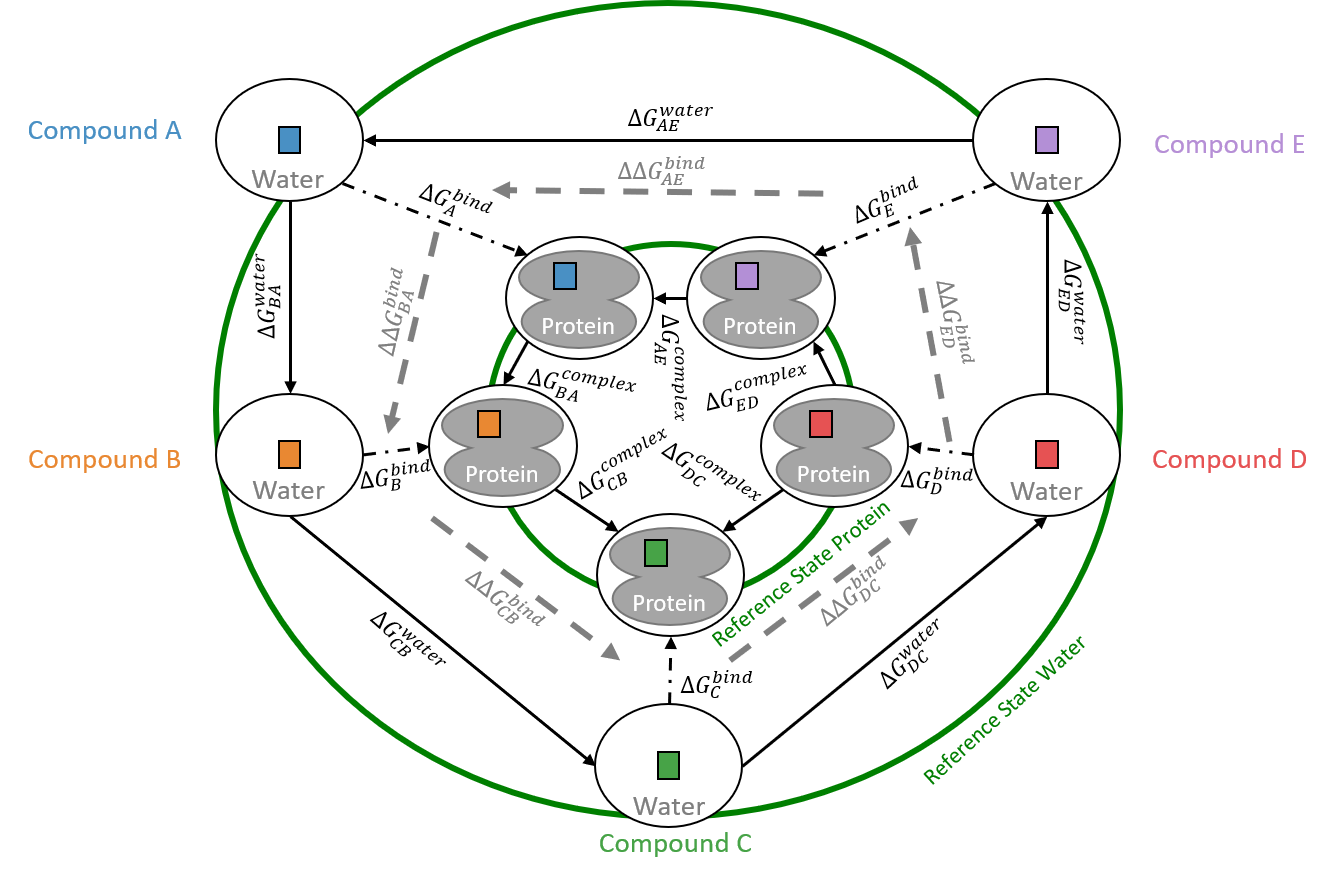
\includegraphics[width=\columnwidth]{fig/intro/State_graph.png}
    \caption{State graph to calculate relative binding free energies, where the nodes represent specific compounds $A$ - $E$ in a particular environment (water/protein). 
    The connecting (directed) edges describe the transformations from one end state to another. The dashed-dotted arrows denote the direct calculation of the (absolute) binding free energy of compound $i$ to the protein, $\Delta G_{i}^\text{bind}$, whereas solid arrows indicate alchemical transformations between compound $i$ to compound $j$ in a given environment. From the resulting $\Delta G_{ji}^\text{env}$, $\Delta \Delta G^\text{bind}_{ji}$ can be calculated and compared with the value obtained from the difference of the experimentally determined $\Delta G_{i}^\text{bind}$ (gray dashed arrows).
    In pathway-dependent methods, each edge between two end states is calculated separately. With (RE-)EDS, all end states in a given environment can be considered simultaneously in a single simulation of a reference state (green circles).}
    \label{fig: StateGraph}
\end{figure}

%The advantage of pathlessness
An attractive and more efficient alternative to path-dependent methods is to simulate a reference state, which includes all $N$ end states simultaneously, without the specification of pathways (green rings in Figure \ref{fig: StateGraph}). Such a reference state is provided by the enveloping distribution sampling (EDS) \cite{Christ2007, Christ2008, Christ2009a, riniker2011} method. The EDS reference state can be further tuned for optimal sampling with parameters. Note that cycle closure is guaranteed by definition in this approach.
%
In order to enhance sampling further, combinations of EDS with enhanced sampling methods were developed such as replica-exchange EDS (RE-EDS) \cite{Lee2014, Sidler2016, Sidler2017} and accelerated EDS \cite{Perthold2018, Perthold2020}.

%conclusion:
In this study, we present an improved automated workflow for RE-EDS simulations that was restructured into two phases. The first phase aims to automatically estimate method parameters that otherwise had to be provided by the user. The second phase automatically optimizes the estimates from the first phase to retrieve a robust parameter set. The final production phase calculates the relative binding free energies of multiple ligands from a single simulation per environment. 
The robustness and versatility of the RE-EDS workflow are demonstrated on a series of five inhibitors of human checkpoint kinase 1 (CHK1) \cite{Huang2012}.
These ligands were selected by Wang \textit{et al.} \cite{Wang2017} as a challenging benchmarking set for FEP calculations since the changes between these ligands exemplify different types of core-hopping transformations (i.e. ring size change, ring opening/closing, and ring extension). Special soft bond-stretching terms were developed to be able to handle these transformations \cite{Wang2017}. In contrast to many other methods, no such special soft bonds are required with RE-EDS as we can use a ``dual topology'' approach \cite{Riniker2011} in a straightforward manner. 


%================================================================================
\section{Theory}
%================================================================================

%------------------------------------------------------------
\subsection{Alchemical Free-Energy Calculations}
%------------------------------------------------------------



The goal of path-dependent alchemical free-energy calculations is
to evaluate the free-energy difference $\Delta G$
between two states $A$ and $B$ of a molecular system,
by introducing a coupling scheme relying on a parameter $\lam$,
and sampling along the so-defined $\lam$-path.
%
The two states have the same number $3N$ of degrees of 
freedom, but distinct Hamiltonian functions $\ham_A(\xv)$ and $\ham_B(\xv)$,
respectively, where $\xv = (\rv,\pv)$ is the $6N$-dimensional
phase-space vector representative of a microscopic system configuration, $\rv$ 
and $\pv$ being the corresponding coordinate and momentum vectors.
%
The coupling parameter is introduced into a hybrid Hamiltonian 
$\ham(\xv;\lam)$ 
satisfying the boundary conditions
$\ham(\xv;0)=\ham_A(\xv)$ and $\ham(\xv;1)=\ham_B(\xv)$,
where the semi-colon indicates a parametric dependence.
%
%
%Examples of methods involving the coupling-parameter approach are 
%multi-configuration\cite{ST91.1} thermodynamic integration\cite{KI33.1,KI34.2,KI35.1} (MCTI or, simply, TI)
%and multi-configuration\cite{JO08.3} free-energy perturbation\cite{ZW54.1,MA95.2,LI96.1,MA99.10,SC99.3,RA12.6,RA17.5,BO17.2} (MC-FEP or, simply, FEP)
%along with their HRE\cite{SU99.1,FU02.2,ZH16.2}/HRP\cite{IT13.1,IT13.2,YA17.2} variants, as well as $\lam$-dynamics\cite{KO96.1,DA01.7,GU03.1,KN09.1,KN11.2,DO11.2,AR15.2,HA17.1} ($\lam$D),
%along with its coordinate-transformed or/and $\lam$-biased variants\cite{GU98.1,GU98.2,SO01.1,WU11.1,KN11.2,DO11.2,KN11.1,ZH12.3,DO13.1,BI14.1,BI14.2,BI15.1,BI15.2} ({\em e.g.} the $\lam$-LEUS scheme\cite{BI14.1,BI14.2,BI15.1,BI15.2}).
%
\revphildel{[-- Redundant paragraph removed --]}
%



Since the proposed CBTI scheme encompasses features of both $\lam$D and TI,
these two approaches are summarized briefly in the \radd{next two subsections.
The following three subsections then describe in turn
the basis of the CBTI scheme, 
its free-energy estimator 
and the application of a biasing potential.}



%------------------------------------------------------------
\subsection{$\lam$-Dynamics ($\lam$D)}
%------------------------------------------------------------


In the $\lam$D scheme\cite{KO96.1,DA01.7,GU03.1,KN09.1,KN11.2,DO11.2,AR15.2,HA17.1}, 
the coupling parameter $\lam$ is assigned a mass
$m_\lam$ and a momentum $p_\lam$, and considered to be an additional
pseudo-conformational degree of freedom of the system.
%
The Hamiltonian of the extended system is defined as
%
\beq{lam_dyn_ext_ham}
  \ham^\star(\xv,\lam) = \ham(\xv;\lam) + \frac{p_\lam^2}{2m_\lam} \ ,
\eeq
%
where the star refers to an extended system in which $\lambda$ 
is now a variable and no longer a parameter 
(thus the replacement of the semi-colon by a comma).
%
This leads to the additional equation of motion
%
\beq{lam_dyn_eq_mot}
  \ddot{\lam} = \frac {\dot{p}_{\lam}} {m_{\lam}} 
              = -\frac {1} {m_{\lam}} 
                 \frac {\partial\ham(\xv;\lam)} {\partial\lam}
\eeq
%
for propagating the $\lam$-variable, \radd{where a dot over a variable indicates its time derivative}.
%


The free-energy difference $\Delta G$
between the two physical end-states can then in principle be
calculated based on a single thermostated MD simulation 
of the extended system, as
%
\beq{lam_dyn_dg}
  \Delta G = 
      - \frac{1}{\beta}\ln\frac{\left\langle \delta(\lam - 1)\right\rangle^\star}
      {\left\langle \delta(\lam)\right\rangle^\star} \ ,
\end{equation}
%
where 
$\beta=(k_BT)^{-1}$, 
$k_B$ being the Boltzmann constant and $T$ the absolute temperature,
$\delta$ is the Dirac delta function, 
and $\langle\cdot\cdot\cdot\rangle^\star$ denotes ensemble averaging 
for the extended system (\ie{} over the joint trajectories of $\xv$ and $\lam$).
%
\revphil{In practice, the $\delta$-functions in \refeq{lam_dyn_dg} must be replaced
      by two finite end-state bins ($\lambda$-cutoff), sufficiently large
      for proper statistics but also sufficiently small for avoiding 
      distortions due to averaging at the end-states\cite{KN11.1}.}
%
\revphildel{[-- Redundant paragraph removed --]}
%
%There are, however, a number of important practical issues 
%to be addressed if this scheme is to be accurate and efficient\cite{BI14.1}:
%%
%($i$) the variations of $\lam$ must be restricted to the range $[0,1]$ between the two physical end-states\cite{KO96.1};
%($ii$) the mass and thermostat-coupling scheme of the $\lam$-variable must be chosen appropriately
%      to ensure a correct temperature for this variable\cite{BI15.1};
%($iii$) the sampling along $\lam$ must generally be adjusted
%      to ensure adequate sampling of the A and B states
%      with a sufficient number of interconversion transitions\cite{BI14.1};
%($iv$) the $\delta$-functions in \refeq{lam_dyn_dg} must be replaced
%      by two finite end-state bins ($\lambda$-cutoff), sufficiently large
%      for proper statistics but also sufficiently small for avoiding 
%      averaging distortions at the end-states\cite{KN11.1}. %
%%
%Different implementation variants of $\lambda$D address these
%issues in a variety of ways, including the use of
%coordinate transformations\cite{KN11.2,DO11.2,WU11.1,KN11.1,DO13.1,ZH12.3,BI14.1,BI15.2},
%memory-based biasing potentials,\cite{GU98.1,GU98.2,SO01.1,WU11.1,BI14.1,BI15.2}
%separate thermostat coupling of the $\lam$-variable\cite{BI14.1,BI15.1,BI15.2},
%and 
%alternative free-energy estimators\cite{LU04.3,SH05.6,KA05.1,KA06.6,FA09.4,KA12.5,TA12.1,DI17.5,ZH17.6}.



%------------------------------------------------------------
\subsection{Thermodynamic Integration (TI)}
%------------------------------------------------------------


In the original TI scheme\cite{KI33.1,KI34.2,KI35.1}, a set of 
$K$ replicas of the system are simulated in parallel at fixed predefined 
$\lam$-values in the range $[0,1]$.
Since the replicas are entirely decoupled 
from each other, the simulations
can be performed serially as well. However, TI extensions 
including the HRE scheme\cite{SU99.1,FU02.2,ZH16.2} and the HRP scheme\cite{IT13.1,IT13.2,YA17.2}
introduce a coupling in the form of $\lam$-value exchanges,
in which case the simulations must really be carried out in parallel.
The same will apply to the proposed CBTI scheme, where the coupling involves a synchronization of
the dynamical $\lam$-variations. 


Considering all replicas $k=0 \dots K-1$ as the members of a replica system,
one may note the corresponding $6K\mkern-3mu\times\mkern-3mu N$-dimensional phase-space vector
as $\Xv=\{\xv_k\}$ and the corresponding $K$-dimensional vector containing the fixed $\lam$-values as 
$\lamv=\{\lam_k\}$.
%
In plain TI, the Hamiltonian of the replica system is defined as
%
\beq{ti_rep_ham}
  \ham^\dagger(\Xv;\lamv) = \sum_{k=0}^{K-1} \ham(\xv_k;\lam_k) \ ,
\eeq
%
where the dagger refers to a replica system,
and $\lamv$ is here a parameter vector (thus the semi-colon).
Because the Hamiltonian of \refeq{ti_rep_ham} involves no coupling 
term  between the replicas, the dynamics of a replica $k$
is independent from that of the other replicas and
solely depends on $\lam_k$.


The free energy difference $\Delta G$
between the two states can then be
calculated based on a single thermostated MD simulation 
of the replica system, as
%
\begin{multline}
  \label{eq:ti_formula}
  \Delta G = 
  \int\limits_0^1 \mathrm{d}\lam' \left\langle \frac{\partial{\ham(\xv;\lam)}}{\partial \lam} \right\rangle_{\lam'} 
    \approx
    \sum_{k=0}^{K-1}  w_k \left\langle \frac{\partial{\ham^\dagger(\Xv;\lamv)}}{\partial \lam_k} \right\rangle^\dagger\\ 
    = 
    \sum_{k=0}^{K-1}  w_k \left\langle \frac{\partial{\ham(\xv_k;\lam_k)}}{\partial \lam_k} \right\rangle^\dagger \ ,
\end{multline}
%
where 
the $w_k$ are quadrature weights for the numerical integration\cite{JO10.2,BR11.5,BR11.6},
$\langle\cdot\cdot\cdot\rangle_{\lam}$ denotes ensemble averaging 
for a single system \radd{(\ie{} over $\xv$) at the given $\lam$ value},
and
$\langle\cdot\cdot\cdot\rangle^\dagger$ denotes ensemble averaging 
for the replica system (\ie{} over $\Xv$).


\revphil{In the above form, TI has long been the workhorse of alchemical free-energy calculations.
%
The method is extremely robust in the sense 
that the accuracy of the calculated $\Delta G$
%free-energy change 
can always be systematically
improved (more $\lambda$-points, longer equilibration or/and sampling times).
However, it is not necessarily the most 
%practical and 
efficient 
method to determine $\Delta G$ up to a certain accuracy,
due to possible sub-optimalities in
the coupling scheme\cite{CR86.1,BL04.2,PH11.1,PH12.1,NA14.1,NA15.3},
the protocol design\cite{ME93.3,HU16.7,ME17.1,SU17.3,DA18.1}
the free-energy estimator\cite{LU04.3,SH05.6,SH08.7,FA09.4,TA12.1,DE16.9,DI17.5,ZH17.6},
and
the orthogonal sampling\cite{WO03.1,WO03.2,KH10.1,KH11.2,BI15.1}.
}
\revphildel{[-- Redundant paragraph removed --]}




%In the above form, TI has long been the workhorse 
%of alchemical free-energy calculations.
%%
%In practice, in addition to the choice of a coupling scheme\cite{CR86.1,BL04.2,PH11.1,PH12.1,NA14.1,NA15.3},
%a TI calculation requires the definition of a protocol including:
%($i$) the number $K$ and distribution (spacing) of the $\lambda$-points considered;
%($ii$) the initial configurations, equilibration times and sampling times
%    selected for each $\lambda$-point;
%($iii$) the choice of a quadrature scheme for the numerical integration.
%%
%The accuracy of the calculation will depend on the selection of these 
%parameters, the optimization of which may represent a non-trivial and 
%time-consuming task\cite{ME93.3,HU16.7,ME17.1,SU17.3,DA18.1}.
%%
%Thus, even though TI is extremely robust in the sense 
%that the accuracy of the calculated free-energy change can always be systematically
%improved (more $\lambda$-points, longer equilibration or/and sampling times),
%it is not necessarily the most efficient method to determine 
%$\Delta G$ up to a certain accuracy.
%
%Many improvements have been proposed for the TI scheme
%over the years.
%%
%Most prominently, the inclusion of $\lam$-exchanges in 
%%HRE\cite{SU99.1,FU02.2,ZH16.2}/HRP\cite{IT13.1,IT13.2,YA17.2} 
%\radd{the HRE scheme\cite{SU99.1,FU02.2,ZH16.2} and the HRP scheme\cite{IT13.1,IT13.2,YA17.2}}
%permits to 
%circumvent orthogonal barriers\cite{WO03.1,WO03.2,KH10.1,KH11.2}, a feature also shared by $\lambda$D schemes\cite{BI15.1}, and
%the use of alternative free-energy estimators like the
%EXTI\cite{DE16.9} scheme or the MBAR\cite{SH08.7} scheme permits to improve the statistical efficiency.



%------------------------------------------------------------
\subsection{Conveyor Belt Thermodynamic Integration (CBTI)}
%------------------------------------------------------------


The proposed CBTI scheme encompasses features of both $\lam$D and TI.
%
Similarly to TI, it is based on the simulation of a replica system involving 
$K$ copies of the molecular system of interest, where $K$ is taken to be even.
%
And similarly to $\lam$D, the individual replicas are extended 
systems, for which the associated $\lam_k$-variable is allowed to evolve
along the simulation.
%
However, the evolutions of these $\lam_k$-variables are not independent. 
They are coupled to each 
other by means of a sequence of hard constraints,
 so that they follow the course of a conveyor belt (CB).
Thus, they are entirely determined by a single dynamical
variable $\Lamb$, following 
the scenario depicted in \reffig{scheme} and discussed
in the Introduction section.



The variable $\Lamb$ is a continuous real variable
representing the overall advance of the CB, successive multiples
of $2\pi$ corresponding to as many full rotations.
%
%
Given $\Lamb$ and $K$, the $\lam$-value $\lam_k$ associated with a system $k$ on the CB
is obtained as
%
\beq{cb_lam_of_big_lam}
  \lam_k(\Lamb) = \zeta\left( \Lamb + k \Delta\Lamb  \right) \ ,
\eeq
%
\radd{with
\beq{delta_lamb}
\Delta\Lamb = 2\pi K^{-1} .
\eeq
}
\radd{Here, the function $\zeta$} is a continuous and periodic zig-zag function of period $2\pi$ and image range $[0,1]$,
defined over the reference period $[0,2\pi)$ as
%
\beq{zigzag_fct}
  \zeta(\theta) = \left\{
                    \begin{array}{ll}
                       \pi^{-1}\theta & \mathrm{if}\ \theta < \pi \\
                       2-\pi^{-1}\theta & \mathrm{if}\ \theta \geq \pi \\
                    \end{array} 
                  \right. \ \ \mathrm{for}\ \theta\in[0,2\pi) \ ,
\eeq
%
where the $[\cdot,\cdot)$ indicates an interval that is open to the right side, {\em e.g.} $[0,2\pi)$ includes $0$ but excludes $2\pi$.
%
\radd{An advance of the CB by $\Delta\Lamb$}
%
corresponds to a cyclic permutation of the $K$ replicas, each system moving by 
one position forward along the CB, \ie
$\lam_k(\Lamb+\Delta\Lamb) = \lam_{k+1}(\Lamb)$
for $k<K-1$, along with
$\lam_{K-1}(\Lamb+\Delta\Lamb) = \lam_0(\Lamb)$.
%
For this reason, the increment $\Delta \Lamb$ will be further referred to 
as one shift of the CB.
%
The system $k=0$ can be viewed as a reference system,
as $\lambda_0=\pi^{-1}\Lambda$ for $0\leq\Lambda<\pi$
and $\lambda_0=2-\pi^{-1}\Lambda$ for $\pi\leq\Lambda<2\pi$.
%
Since $K$ is chosen to be even, an increase of $\Lambda$
always corresponds to an increase of $\lambda_k$
for half of the systems (forward-moving side of the CB)
and a decrease of $\lam_k$ for the other half of the systems
(backward-moving side of the CB). This choice also implies that 
$\Lamb$-values which are integer multiples of the
CB shift $\Delta \Lamb$ 
correspond to situations where there is 
one system in state $A$ and one system in state $B$.
%
Since an advance of the CB variable by $2\pi$
leaves the replica system invariant, 
the variable $\Lamb$ will commonly be refolded into the 
reference period $[0,2\pi)$ when illustrating the
results of the CBTI method.

The Hamiltonian of the extended replica system is defined as
%
\beq{cb_ext_rep_ham}
  \ham^{\dagger\star}(\Xv,\Lamb) = \ham^\dagger(\Xv;\lamv)  +  \frac{p_\Lamb^2}{2m_\Lamb} 
  \quad \text{with} \quad \lamv=\lamv(\Lamb),
\eeq
%
%
where $\ham^{\dagger}$ is defined as in TI by \refeq{ti_rep_ham}
and $\lamv(\Lamb)$ by \refeq{cb_lam_of_big_lam}.
%
In analogy with \refeq{lam_dyn_eq_mot}, the resulting equation of motion for $\Lamb$ reads
%
\beq{cb_big_lam_eq_mot}
  \ddot{\Lamb} = \frac {\dot{p}_{\Lamb}} {m_{\Lamb}} 
              = -\frac {1} {m_{\Lamb}}  \frac {\partial\ham^\dagger(\Xv;\lamv)} {\partial \Lamb} 
\eeq
%
where
%
\begin{align}
  \label{eq:cb_big_lam_eq_mot_der}
   \frac{\partial\ham^\dagger(\Xv;\lamv)}{\partial\Lamb}
        &= \sum_{k=0}^{K-1} \frac {\partial\ham(\xv_k;\lam_k)} {\partial \lam_k} \frac{\mathrm{d} \lam_k}{\mathrm{d} \Lamb}\nonumber \\
        &= \sum_{k=0}^{K-1} \frac {\partial\ham(\xv_k;\lam_k)} {\partial \lam_k} \zeta'\left( \Lamb + 2\pi K^{-1} k \right) \ .
\end{align}
%
Here, the function $\zeta'$ is the derivative of the zig-zag function of \refeq{zigzag_fct}, 
given over the reference period $[0,2\pi)$ by
%
\beq{zigzag_der}
  \zeta'(\theta) = \left\{
                    \begin{array}{ll}
                       \pi^{-1} & \mathrm{if}\ \theta < \pi \\
                       -\pi^{-1} & \mathrm{if}\ \theta \geq \pi \\
                    \end{array} 
                  \right. \ \ \mathrm{for}\ \theta\in[0,2\pi) \ .
\eeq
%
Formally, the derivative is not defined when $\theta$
is an integer multiple of $\pi$, \ie{} for a system that is exactly 
in one of the physical end-states $A$ or $B$. In this case, the value of $\zeta'$ has been arbitrarily set to 
$\pi^{-1}$ for even multiples and $-\pi^{-1}$ for odd multiples.
This has a negligible impact in practice, as it only concerns a series
of infinitesimal points over the entire $\Lamb$-range, 
\ie{} infinitesimally few configurations along a CBTI simulation.
%
\revphil{For example, when using double-precision floating-point arithmetics
(including denormalized numbers),
their probability of occurrence is on the order of 10$^{-324}K$ 
({\em i.e.} a single expected occurrence over a simulation lasting about 10$^{292}K^{-1}$
times the age of the universe with a 2 fs timestep).
}
%
Neither does going over the discontinuity within a timestep represent a source of non-conservativeness. The concerned replica
will merely bounce back the corresponding physical end-state with a reversion of its velocity, akin to a particle reflected elastically
by a hard wall (delta-function force).
%
If desired, these \revphil{exceptional points could be handled
more formally by altering} the definition of $\zeta$,
\revphil{{\em e.g.} by smoothing its tips in a narrow range around $0$ and $\pi$}.


The $\lam_k$-dynamics of the individual systems is entirely
specified by \refeq{cb_big_lam_eq_mot} to propagate $\Lamb$
along with  \refeq{cb_lam_of_big_lam} to calculate the $\lam_k$-values from the current $\Lamb$.
Alternatively, one may write an equation of motion for the $\lambda_k$-variables of the 
individual replicas by combining the two equations (along with \refeq{cb_big_lam_eq_mot_der}) as
%
\begin{align}
  \label{eq:cb_lam_eq_mot}
  \ddot{\lam}_k &= \ddot{\Lamb} \frac{\mathrm{d} \lam_k}{\mathrm{d} \Lamb} + \dot{\Lamb}^2 \frac{\mathrm{d^2} \lam_k}{\mathrm{d} \Lamb^2} \nonumber\\
                &= -\frac {1} {m_{\Lamb}} \left( 
                       \sum_{l=0}^{K-1} \frac {\partial\ham(\xv_{l};\lam_{l})} {\partial \lam_{l}} \zeta'\left( \Lamb + 2\pi K^{-1} l \right) 
                       \right) \nonumber  \\
                   & \qquad \zeta'\left( \Lamb + 2\pi K^{-1} k \right) \ .
\end{align}
%
%
Note that the term in $\dot{\Lamb}^2$ vanishes since the second derivative $\zeta''$ of $\zeta$
is zero (except at the \radd{exceptional} singular points). However, it should not be overlooked 
if one decides to use a different function $\zeta$.
%
Introducing the vector $\Dv$ and the symmetric $\Lamb$-dependent matrix $\Cmat$ defined 
by their components as
%
\begin{multline}
  \label{eq:cb_def}
 D_k = \frac{\partial\ham(\xv_{k};\lam_{k})}{\partial \lam_{k}}
\ \ \ \mathrm{and}\\
C_{kl}(\Lambda) = \pi^2 \zeta'\left( \Lamb + 2\pi K^{-1} k \right) \zeta'\left( \Lamb + 2\pi K^{-1} l \right) \ ,
\end{multline}
%
\refeq{cb_lam_eq_mot} can be rewritten in an elegant matrix form as
%
\beq{cb_lam_eq_mot_mat}
  \ddot{\lamv} = -\frac {\Cmat(\Lamb)} {\pi^2 m_{\Lamb}}  \Dv \ .
\eeq
%
The elements of the symmetric matrix $\Cmat$
are either -1 (pair of systems currently on opposite sides of the CB,
and thus moving in opposite directions) or +1
(pair of systems currently on the same side of the CB, and thus moving in the same direction). The diagonal elements
are all +1, and the other +1 values surround the diagonal (line- and column-wise),
the rest being -1 values.
Because $K$ is even, the two types of values 
are always equally represented in the matrix, 
specific locations
depending on $\Lamb$.
%
Note that the variable $\Lamb$ itself still needs to be explicitly propagated
using \refeq{cb_big_lam_eq_mot}.

%%\revphil{Discussion in page 16-18 a little hard to get through.}

For a given configuration $\Xv$ of the replica system, the Hamiltonian
$\ham^\dagger$ of \refeq{ti_rep_ham} (together with \refeq{cb_lam_of_big_lam}) is periodic in $\Lamb$ 
with a period $2\pi$ corresponding to a full rotation of the CB.
%
However, because the Hamiltonians of the individual replicas are 
identical, upon ensemble averaging over $\Xv$, 
one expects the calculated properties to be periodic over $\Lamb$ 
with a smaller period $\Delta \Lamb$, corresponding to one shift of the CB.
%
\revphil{
This is in particular the case for the probability distribution $P(\Lamb)$
along $\Lamb$ and the associated free-energy profile $G_{\Lamb}(\Lamb)$,
given by
%
%\begin{align}
%\label{eq:fre_prof_lam_def}
%%\beq{fre_prof_lam_def}
%  G_{\Lamb}(\Lamb) &= G_{\Lamb}(0) +
%      \int\limits_0^\Lamb \mathrm{d}\Lamb' \left\langle \frac{\partial{\ham^{\dagger}(\Xv;\lamv)}}{\partial \Lamb} \right\rangle^{\dagger}_{\Lamb'} \\ \nonumber
%    &=  G_{\Lamb}(0) + \sum_{k=0}^{K-1}  \left[ G(\lam_k(\Lamb)) - G(\lam_k(0))\right] \quad \text{with} \  \lamv=\lamv(\Lamb) \ ,
%\end{align}
%
\begin{align}
  \label{eq:fre_prof_lam_def}
  G_{\Lamb}(\Lamb) &= G_{\Lamb}(0) +
      \int\limits_0^\Lamb \mathrm{d}\Lamb' \left\langle \frac{\partial{\ham^{\dagger}(\Xv;\lamv)}}{\partial \Lamb} \right\rangle^{\dagger}_{\Lamb'} \nonumber \\
    &=  \tilde{G}_{\Lamb}(0) + \sum_{k=0}^{K-1} G(\lam_k) \quad \text{with} \  \lamv=\lamv(\Lamb) \ ,
\end{align}
%
where $\lamv(\Lamb)$ is defined by \refeq{cb_lam_of_big_lam},
$\langle\cdot\cdot\cdot\rangle^{\dagger}_{\Lamb}$ denotes ensemble averaging 
for the replica system (\ie{} over $\Xv$) at the given $\Lamb$ value,
and the second equality follows from \refeqs{ti_rep_ham} and \refeqn{ti_formula}
(the unknown constant $\tilde{G}_{\Lamb}(0)$ 
is equal to $G_{\Lamb}(0)$ increased by a sum of $-G(\lam_k(0))$
offsets).
%
}
%


\radd{Owing to this periodicity over a smaller interval}, it is convenient to introduce a fractional advance variable $\tilde{\Lamb}$
defined as
%
\beq{tilde_lamb_def}
   \tilde{\Lamb} = \gamma( \Lamb, \Delta \Lamb ),
\eeq
%
where
%
\beq{gamma_def}
   \gamma(\theta,\theta_o)
     = \theta_o  \left( \theta_o^{-1}\theta - \lfloor \theta_o^{-1}\theta \rfloor \right)
\eeq
%
returns the part of $\theta$ in excess of the closest lower integer multiple of $\theta_o$.
%
In contrast to $\Lamb$, which is an unbounded variable, $\tilde{\Lamb}$ only spans a finite definition interval $[0,\Delta \Lamb)$.
%
At full convergence, 
any average property binned as a function 
of $\Lambda$ over the interval $[0,2\pi)$ will 
consist of $K$ successive repeats of the same property binned
as a function of $\tilde{\Lambda}$ over its definition interval $[0,\Delta \Lamb)$, as observed in \reffig{scheme:ene:sinus} for the free energy \radd{$G_{\Lamb}(\Lamb)$}.
%
Accordingly, in the absence of full convergence
along $\Lambda$, binning as a function of $\tilde{\Lambda}$
over the interval $[0,\Delta \Lamb)$ followed by $K$-fold replication
provides an efficient way to construct a more accurate representation of any 
$\Lambda$-resolved average quantity. In fact, the definition interval of $\tilde{\Lamb}$ could be further halved by noting that, upon ensemble averaging over $\Xv$ and for any $\Lamb$ value that is an integer multiple of $\Delta \Lamb$, a forward move of the CB produces the same result as a backward move of the same magnitude. Consequently, $\Lamb$-resolved average properties are even over successive $2\pi K^{-1}$ intervals, as also observed in \reffig{scheme:ene:sinus} for the free energy
\radd{$G_{\Lamb}(\Lamb)$}. The corresponding information is thus entirely encompassed in an interval of size $\Delta \Lamb /2$.

The normalized probability distribution $p(\lam)$ 
along the coupling variable $\lam$ considering all the replicas is defined by
%
\beq{proba_of_lam}
  p(\lam) = K^{-1} \sum_{k=0}^{K-1} \left\langle \delta(\lam_k-\lam) \right\rangle^{\dagger\star} \ ,
\eeq
%
\radd{where $\langle\cdot\cdot\cdot\rangle^{\dagger\star}$ denotes ensemble averaging 
for the extended replica system (\ie{} over the joint trajectories of $\Xv$ and $\lamv$).}
%
At full convergence, this probability over the interval $[0,1]$
will consist of $K/2$ successive
repeats of the corresponding distribution over the interval $[0,2 K^{-1})$.
%
\radd{More precisely, the distribution $p(\lam)$} is related to the distribution 
$\tilde{P}(\tilde{\Lamb})$ of $\tilde{\Lamb}$ over interval $[0,\Delta \Lamb)$
as
%
%\revdavid{Shouldn't there be a factor, \ie
\beq{proba_of_lam_from_that_of_big_lam}
%  p(\lam) = \tilde{P}( \pi \gamma( \lam, 2 K^{-1} )  ) \ .
  p(\lam) = \Delta \Lamb\,\tilde{P}( \pi \gamma( \lam, \pi^{-1}\Delta\Lamb )  )  \ .
\eeq
%}
%
%\beq{proba_of_lam_from_that_of_big_lam}
%%  p(\lam) = \tilde{P}( \pi \gamma( \lam, 2 K^{-1} )  ) \ .
%  p(\lam) = \tilde{P}( \pi \gamma( \lam, \pi^{-1}\Delta\Lamb )  ) \ .
%\eeq
%
In plain words, this means that $\tilde{P}(\tilde{\Lamb})$ is the relevant quantity
in terms of sampling along the coupling variable $\lam$.
If it is close to uniform over the range $[0,\Delta \Lamb)$,
then $p(\lam)$ will also be close to uniform over the range $[0,1]$.
Here again, it is noted that $p(\lam)$ is also even over the interval $[0,2 K^{-1})$,
and could be mapped to a $\tilde{\Lamb}$ value defined over an interval of size $\Delta \Lamb / 2$ instead of $\Delta \Lamb$ if desired, as

\beq{sym_proba_lam}
  p(\lam) = \left\{
                    \begin{array}{ll}
%                       \tilde{P}(\pi \gamma(\lam, 2 K^{-1})) & \mathrm{if}\ \gamma(\lam, 2 K^{-1}) < K^{-1} \\
                       \Delta \Lamb\,\tilde{P}(\pi \gamma(\lam, \pi^{-1}\Delta\Lamb)) & \mathrm{if}\ \gamma(\lam, \pi^{-1}\Delta\Lamb) < (2\pi)^{-1}\Delta\Lamb \\
%                       \tilde{P}(\pi \gamma(1-\lam,  2 K^{-1})) & \mathrm{otherwise} \\
                       \Delta \Lamb\,\tilde{P}(\pi \gamma(1-\lam,  \pi^{-1}\Delta\Lamb)) & \mathrm{otherwise} \\
                    \end{array} 
                  \right. .
\eeq


\radd{
%------------------------------------------------------
\subsection{CBTI Free-energy Estimator}
%------------------------------------------------------------
}


Due to the constraints coupling the $\lam_k$-values of the
$K$ replicas, the function $p(\lam)$ of \refeq{proba_of_lam}
is by no means a Boltzmann distribution in terms of the single-system
Hamiltonian. In fact, as seen above, it consists at full convergence
of $K/2$ successive repeats of the same even
curve.
In addition, compared to the Boltzmann distribution,
it will be
significantly flatter. On the one hand, the smaller amplitude of variations 
%and the reduced barriers 
are desired, as they will lead to more homogeneous sampling 
and \revphil{are expected to ease transitions along $\Lamb$ 
(up to the limit imposed by the speed of random diffusion)}.
%
%\revphil{
%Page 18: says that 'there is a smaller amplitude of variations and
%reduced barriers', but it's not clear dynamics are faster, since the
%dH/dl force is slowed down by (averaged). I think this is eventually
%explained by the fact that it becomes nearly diffusive behavior, but
%perhaps this can be brought up sooner.
%}
%
%
On the other hand, it is no longer possible to evaluate 
the free-energy difference $\Delta G$
directly from $p(\lam)$ in analogy with the $\lam$D expression of \refeq{lam_dyn_dg}.
%
However, since the dynamics remains Hamiltonian and the coupling 
between replicas does not
involve the configurational degrees of freedom, the change \radd{from TI to CBTI} does not affect 
the conditional probabilities $\mathcal{P}(\xv | \lam)$. Thus,
configurational ensemble averages sorted by $\lam$-values will remain
identical to those one would obtain from TI \radd{(or from HRE/HRP or $\lam$D)}.
%
As a result, $\Delta G$ can still be obtained 
\radd{by integrating over the average Hamiltonian derivative binned as a function 
of $\lambda$ considering all replicas simultaneously,}
in analogy with the TI expression
of \refeq{ti_formula}.
%
\revphil{Note that the exceptional points of the function $\zeta'$
(discussed previously in the context of \refeq{zigzag_der})
have no influence on the integration, as they represent
finite discontinuities over infinitesimal ranges.
}
%\revphil{SAY THAT DISCONT HAS NO EFFECT
%See Point 6 above. Similar considerations apply to the integration.
%We integrate $\partial\mathcal{H}/\partial\lam$. If the value is off
%at one (or a few) points, the integral is unaffected because the 
%neighborhood of the singularity is infinitesimal and its magnitude
%is finite ({\em i.e.} it is not a $\delta$ function, but just 
%a finite change in the function value).
%}



In practice, \revphil{$\Delta G$} is calculated here based on a single thermostated MD simulation 
of the extended replica system, as
%
\begin{align}
\label{eq:cbti_formula}
  \Delta G &= 
    \int_0^1 \mathrm{d}\lam' K^{-1} \sum_{k=0}^{K-1} \left\langle 
                 \frac{\ham(x_k;\lam_k)}{\partial \lam_k} \delta(\lam_k-\lam')
            \right\rangle^{\dagger\star}\\ \nonumber
   &\approx
%     K^{-1} 
\sum_{j=0}^{J-1}  \left \langle \frac{ \sum_{k=0}^{K-1} \frac{\ham(x_k;\lam_k)}{\partial \lam_k} \alpha(\lambda_k,j;J)}
                              { \sum_{k=0}^{K-1} \alpha(\lambda_k,j;J)}  \right \rangle^{\dagger \star}                                   ,
\end{align}
%
where 
%
\beq{binning_fct}
\alpha(\theta,j;J)=\begin{cases}
1 \qquad \text{if}\ j\leq J\theta < j+1 \\
0 \qquad \text{otherwise}
\end{cases}
\eeq
%
is a binning function  corresponding to a discretization of the $\lam$-interval $[0,1]$ using
$J$ bins. 
%
The approximation in \refeq{cbti_formula} corresponds to a 
simple forward rectangular quadrature, where the Hamiltonian derivative is 
averaged over the $J$ successive bins considering all replicas.
%
Since $\tilde{P}(\tilde{\Lamb})$, and thus $p(\lam)$, will typically be close to homogeneous, $J$ can be taken very large, 
resulting in a negligible quadrature error. 
For example, if $K$ replicas sample $L$ configurations each, the number of data points
per bin will be close to $K L/J$, with limited variations across bins. 
Defining
the maximal allowed value $J_{\mathrm{max}}$ as the highest value of $J$ for which 
empty bins (vanishing denominator in the ensemble average of \refeq{cbti_formula}) never 
occur, a graph of $\Delta G$ evaluated upon increasing $J$ from 1 to $J_{\mathrm{max}}$ 
will rapidly level off to a plateau when quadrature errors become negligible.
%sufficiently small. 
%
\revphil{
Two variants which do not require the specification 
of a number of bins are also proposed in \refsec{CH2C} (\refeqs{cbti_formula_app1} and \refeqn{cbti_formula_average}).}
%
\revphildel{[-- Variants moved to Appendix C --]}



%------------------------------------------------------------
\subsection{CBTI with Memory-based Biasing Potential}
%------------------------------------------------------------

%For a 
When using a large number of replicas, the sampling along $\lam$ afforded by the CBTI scheme will be close to homogeneous. However, for practical reasons (\eg{} number of processors available on a computer node), one may wish to use a small number of replicas. In this case, the sampling homogeneity can be enhanced by addition of a biasing potential. It is sufficient to apply this potential to the fractional advance variable $\tilde{\Lambda}$ over the range $[0,\Delta \Lamb)$. With inclusion of a biasing potential $\mathcal{B}$, \refeq{cb_big_lam_eq_mot} becomes 
%
  \begin{multline}
  \label{eq:cb_big_lam_eq_mot_bias}
  \ddot{\Lamb} = -\frac {1} {m_{\Lamb}} \frac {\partial}{\partial \Lamb} \left ( \ham^\dagger(\Xv;\lamv)  
  + \mathcal{B}(\tilde{\Lamb}) \right) \\ \text{with} \  \lamv=\lamv(\Lamb)\ \text{and}\ \tilde{\Lamb}=\tilde{\Lamb}(\Lamb) \ ,
  \end{multline}
%
where $\mathcal{H}^{\dagger}$ is defined by \refeq{ti_rep_ham}, $\lamv(\Lamb)$ by \refeq{cb_lam_of_big_lam} and $\tilde{\Lamb}(\Lamb)$ by \refeq{tilde_lamb_def}. 


In analogy with the $\lam$-LEUS scheme\cite{BI14.1,BI14.2,BI15.1,BI15.2}, this biasing potential can be expressed as a sum of local grid-based spline functions, built in a LE preoptimization phase and frozen in a subsequent US sampling phase. However, the duration of the LE phase can be considerably reduced compared to a single-system $\lam$-LEUS simulation, considering that $\tilde{P}(\tilde{\Lamb})$ is already close to homogeneity in the absence of biasing and that the support interval is reduced to the $\tilde{\Lamb}$-range $[0,\Delta \Lamb)$. The latter interval can actually be further restricted to $[0,\Delta \Lamb / 2]$ considering the even symmetry of $\tilde{P}(\tilde{\Lamb})$, \ie{} by enforcing an even symmetry of $\mathcal{B}$ as well.

Since the application of a biasing potential that only involves the $\lam_k$-variables does not alter the 
conditional probabilities $\mathcal{P}(\xv|\lam)$, \refeq{cbti_formula} \revphil{(or the variants of \refeqs{cbti_formula_app1} and \refeqn{cbti_formula_average})}
can still be employed without any modification to evaluate the free-energy change. In other words, 
in contrast to the $\lam$-LEUS scheme, the CBTI scheme with the presented TI-like free-energy estimator does not require any reweighting.


%================================================================================
\section{Computational Details}
%================================================================================


\subsection{Validation of the Restraint Selection Algorithm}
To assess the performance of the greedy algorithm for selecting optimal distance restraints between two molecules, it was first tested on toy models. These contained 12 to 30 particles that were randomly distributed in space. The particles were randomly assigned to two entities representing two molecules. A selection of four restraints was performed with no pre-processing steps. Different algorithmic approaches were compared: the developed greedy algorithm, an averaged random selection (100 repetitions), and two brute-force approaches. One of the brute-force approaches maximizes the sum of the restraint midpoint distances between the selected restraints by considering all possible quadruples of restraints explicitly (BF-maxD). The other one maximizes the CHV around the selected restraints (BF-maxCHV), as done for chaining in multi-state systems. Each number of particles was sampled 20 times (using different particle coordinates each time) to provide an uncertainty estimate. The scripts for this validation are available in the example folder of the GitHub repository (\textit{examples/publication/a\_benchmark\_algorithms}).

\subsection{Molecules with Hydration Free Energies}
The algorithm was applied for the calculation of relative hydration free energies $\Delta \Delta G_{\text{hyd}}$ (Figure \ref{fig:thermodynamic_cycle}).
A set of 16 molecules with experimentally available hydration free energies\cite{Wolfenden1987,Rizzo2006,Nicholls2008,Guthrie2009,Guthrie2014,Mobley2014} were selected (Table \ref{tab:SI_moleculelist}). 
The topologies for these molecules were taken from the ATB server.\cite{Stroet2018} The selected molecules are small and possess a ring core. The corresponding pairwise transformations are nevertheless relatively complex, and involve R-group and ring-size changes as well as scaffold hopping-type transformations (e.g. benzene to cyclohexane).

\begin{figure}[h!]
    \centering
    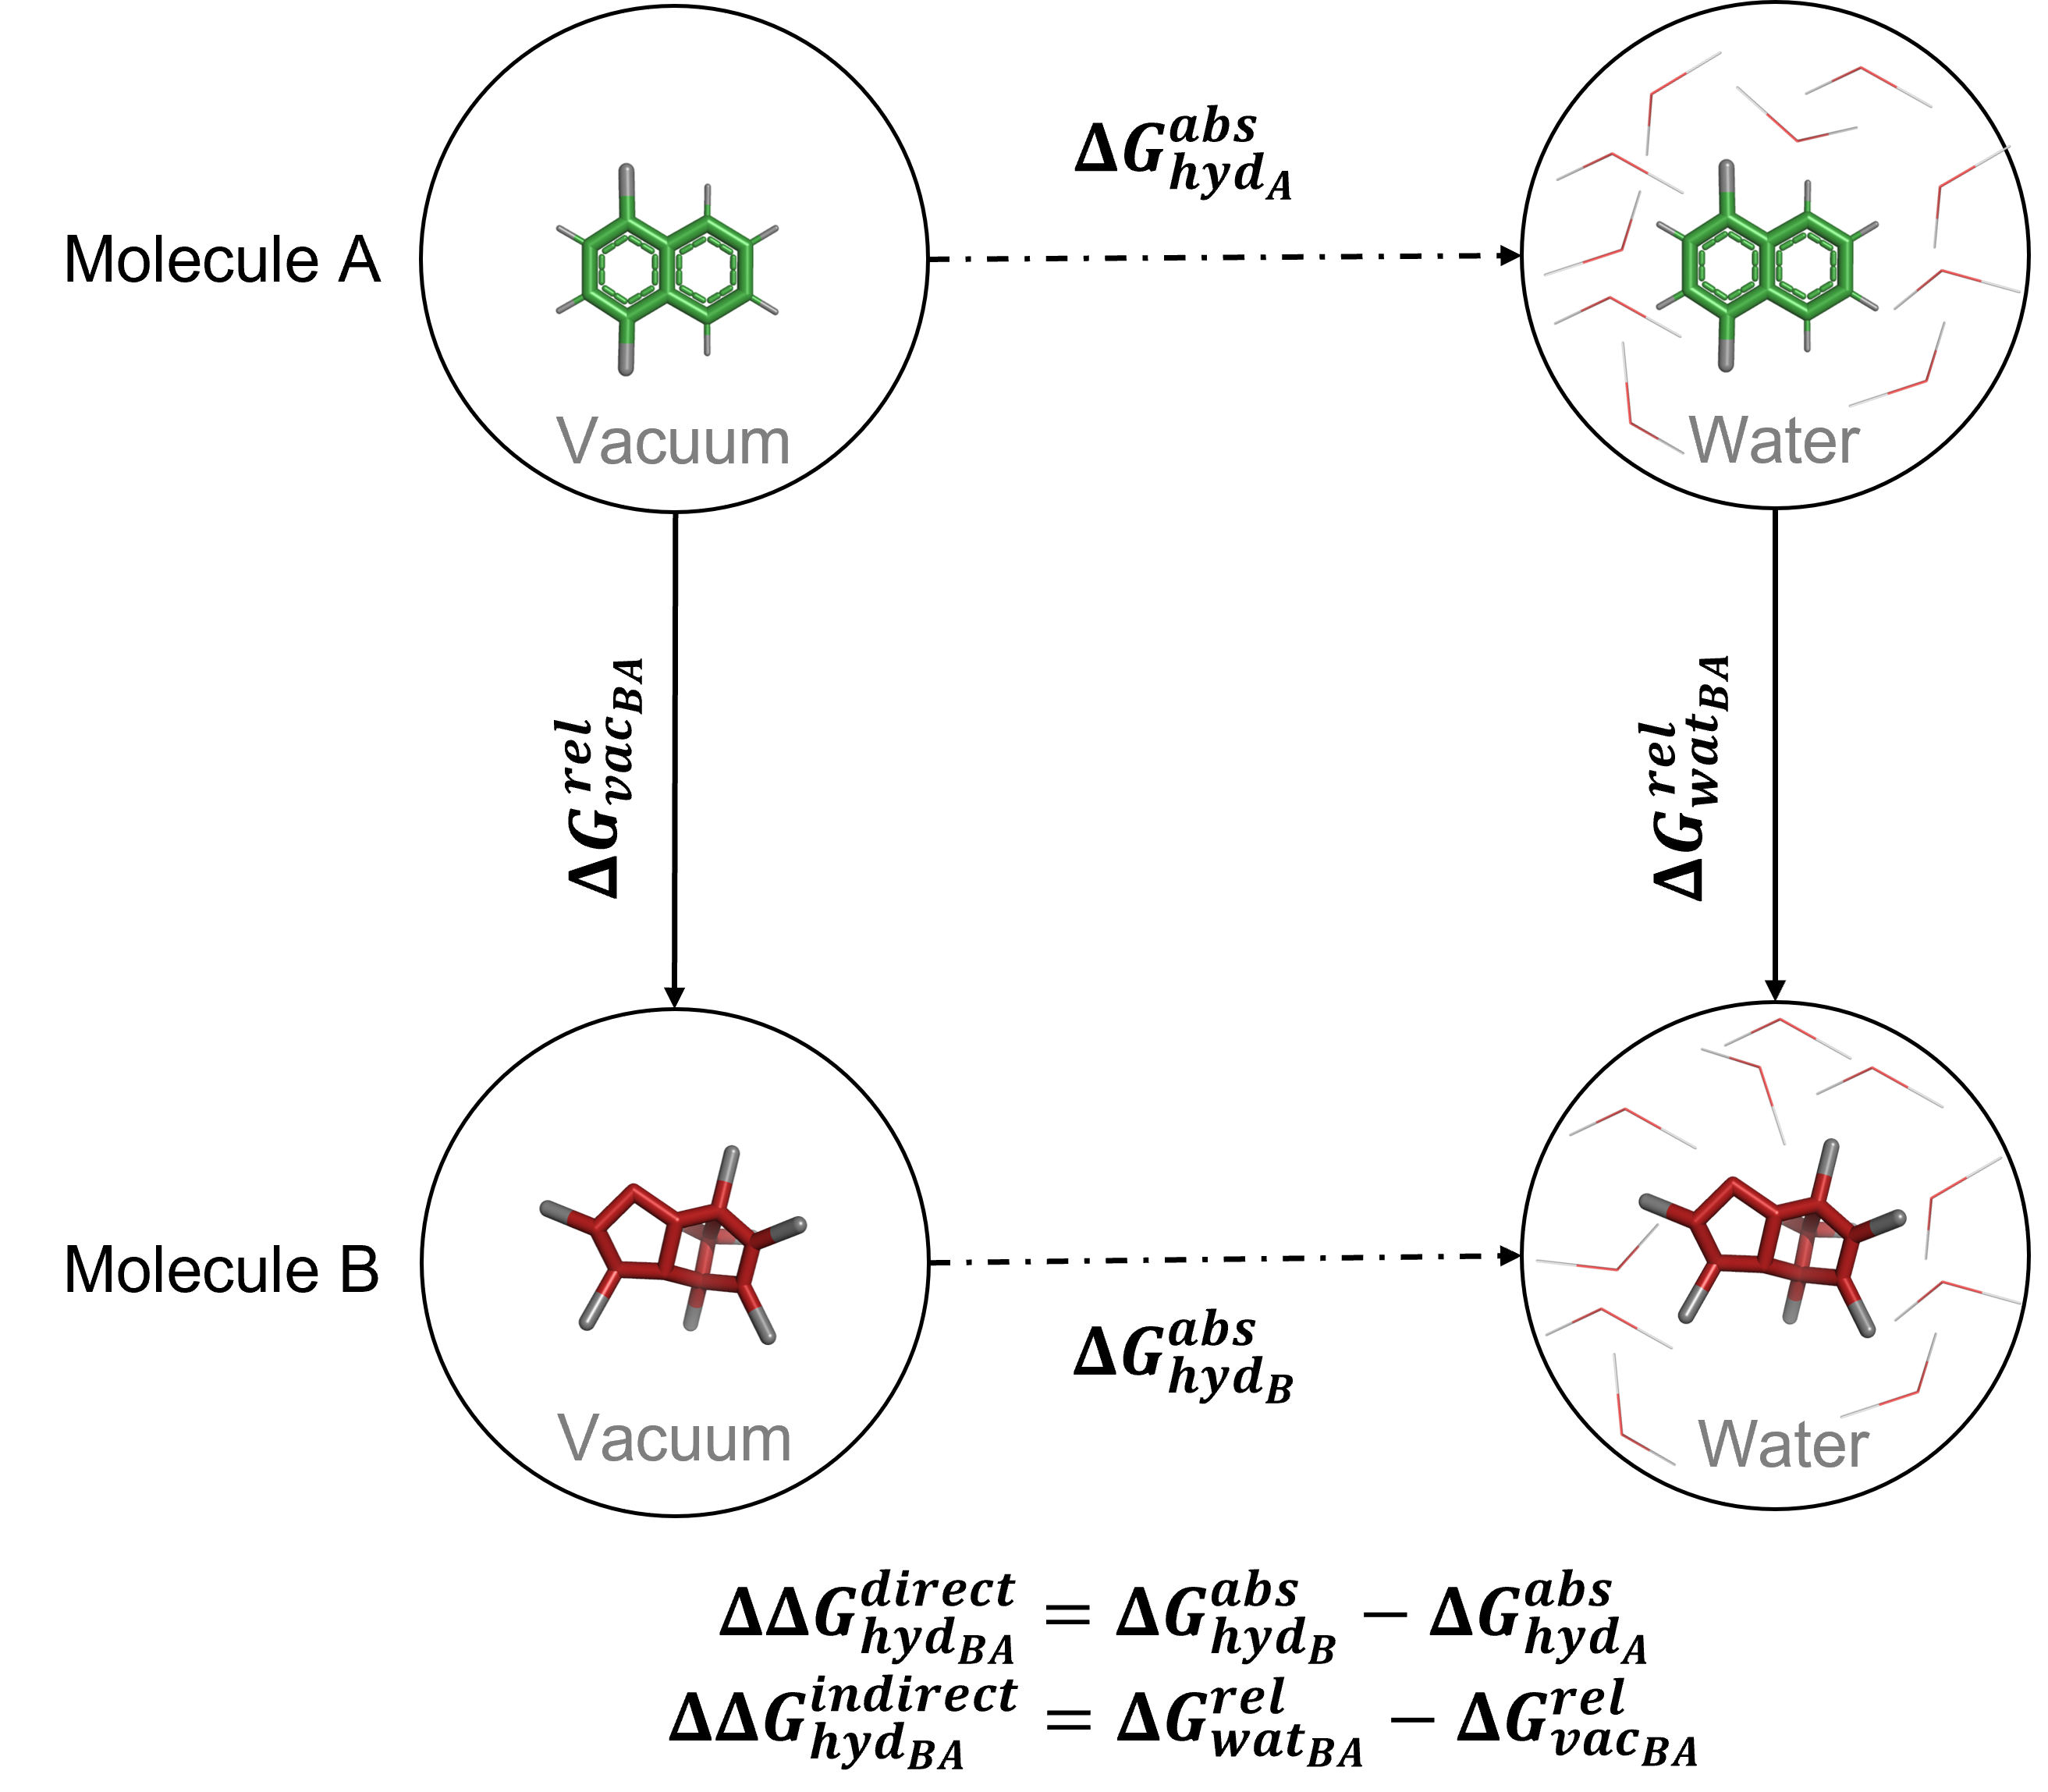
\includegraphics[width=0.8\textwidth]{fig/theory/ThermCycle.png}
    \caption{Thermodynamic cycle for the calculation of relative hydration free energies $\Delta \Delta G_{\text{hyd}_{AB}}$. The direct way to obtain $\Delta \Delta G_{\text{hyd}_{AB}}$ employs two absolute free-energy calculations giving $\Delta G^\text{abs}_{\text{hyd}_A}$ and $\Delta G^\text{abs}_{\text{hyd}_B}$. The indirect way uses two alchemical or relative free-energy calculations giving $\Delta G^\text{rel}_{\text{vac}_{AB}}$ and $\Delta G^\text{rel}_{\text{wat}_{AB}}$.
    }
    \label{fig:thermodynamic_cycle}
\end{figure}

\begin{table}[H]
\caption{Identifier of the ATB server\cite{Stroet2018}, IUPAC name, and canonical SMILES for the 16 molecules with experimental hydration free energies.}\label{tab:SI_moleculelist}
%\scriptsize
\resizebox{\columnwidth}{!}{%
\centering
\begin{tabular}{l | l | l }
Ligand & Identifier & IUPAC name \\
\hline
1 & \_O6T & 1,2-dimethoxybenzene \\
2 & \_O70 & (2R,5R)-2-methyl-5-prop-1-en-2-ylcyclohexan-1-one\\
3 & \_O71 & (1S,5R)-2-methyl-5-prop-1-en-2-ylcyclohex-2-en-1-ol \\ 
4 & \_P8I & cyclopentanone \\
5 & 6J29 & 1-amino-4-hydroxyanthracene-9,10-dione \\
6 & 6KET & 3-methoxyphenol \\
7 & 8018 & (1R,2S,3R,4R,6S,7S)-1,3,4,7,8,9,10,10-octachlorotricyclo[5.2.1.02,6]dec-8-ene \\
8 & E1VB & [1,2,2-Trifluoroethoxy]benzene\\
9 & F313 & 4-methoxyaniline \\
10 & G078 & 1,4-dimethylnaphthalene \\
11 & G277 & cyclohexa-2,5-diene-1,4-dione\\
12 & M030 & 1,3,5-trimethylbenzene \\
13 & M097 & 2-chloroaniline \\
14 & M218 & N-methylaniline \\
15 & S002 & bromomethylbenzene \\
16 & TVVS & pyridine-4-carbaldehyde\\
\end{tabular}
}
\end{table}


Pairwise TI calculations were carried out with a linked dual topology approach for the 16 molecules in a star-like scheme with molecule \textbf{12} as center, resulting in 15 relative hydration free energies (Figure \ref{fig: Pairwise_TI_M030_Graph}).
\begin{figure}[h]
    \centering
    
\includegraphics[width=\textwidth]{fig/methods/StateGraph_TI_2D_enumerated.png}
    \caption{Set of 16 molecules with experimental hydration free energies available \cite{Stroet2018,Wolfenden1987,Rizzo2006,Nicholls2008,Guthrie2009,Guthrie2014,Mobley2014}. The black lines indicate the pairs of molecules for which TI calculations were performed. RestraintMaker was used to select pairwise distance restraints between the central molecule and all others.} 
    \label{fig: Pairwise_TI_M030_Graph}
\end{figure}

\subsection{Simulation Details}
All simulations were carried out using the MD software package GROMOS\cite{Schmid2012} version 1.5.0 (freely available on \textit{http://www.gromos.net}),\cite{Ries2021B} the Python RE-EDS pipeline\\ (\textit{https://github.com/rinikerlab/reeds}) 
and PyGromosTools\cite{Lehner2021}\\ (\textit{https://github.com/rinikerlab/PyGromosTools}). 

In order to compare our results with the absolute hydration free energies reported in the ATB server,\cite{Stroet2018} the same simulation setup was used.
The simple point-charge (SPC) model\cite{Berendsen1981} was employed for water. A single cutoff radius of $1.2$~nm was used for the calculation of the non-bonded interactions. The integration time step was set to $2$~fs and the pairlist was updated every five steps. Long-range nonbonded interactions were calculated using a reaction-field correction\cite{Tironi1995} with $\varepsilon_{\text{rf}}=1$ for the simulations in vacuum and $\varepsilon_{\text{rf}}=61$ for the simulations in water.\cite{Heinz2001} The force constant for the distance restraints was set to $5000$ kJ$/($mol$\cdot$nm$^2)$.

\subsubsection{Thermodynamic Integration}
The topologies and coordinate files of the single states were obtained from the ATB server\cite{Stroet2018} and were merged to pairs using PyGromosTools\cite{Lehner2021}. 
The coordinates of the different single molecules were aligned to each other using the common molecular skeleton of the molecules (only rings), with the \textit{align} function in RDKit\cite{Landrum2021}. After the alignment, RestraintMaker was used to place four restraints with $d_\text{res} = 0.1$~nm (Figures \ref{SIfig: Pairwise_TI_M030_Graph}. 

\begin{figure}[H]
    \centering
    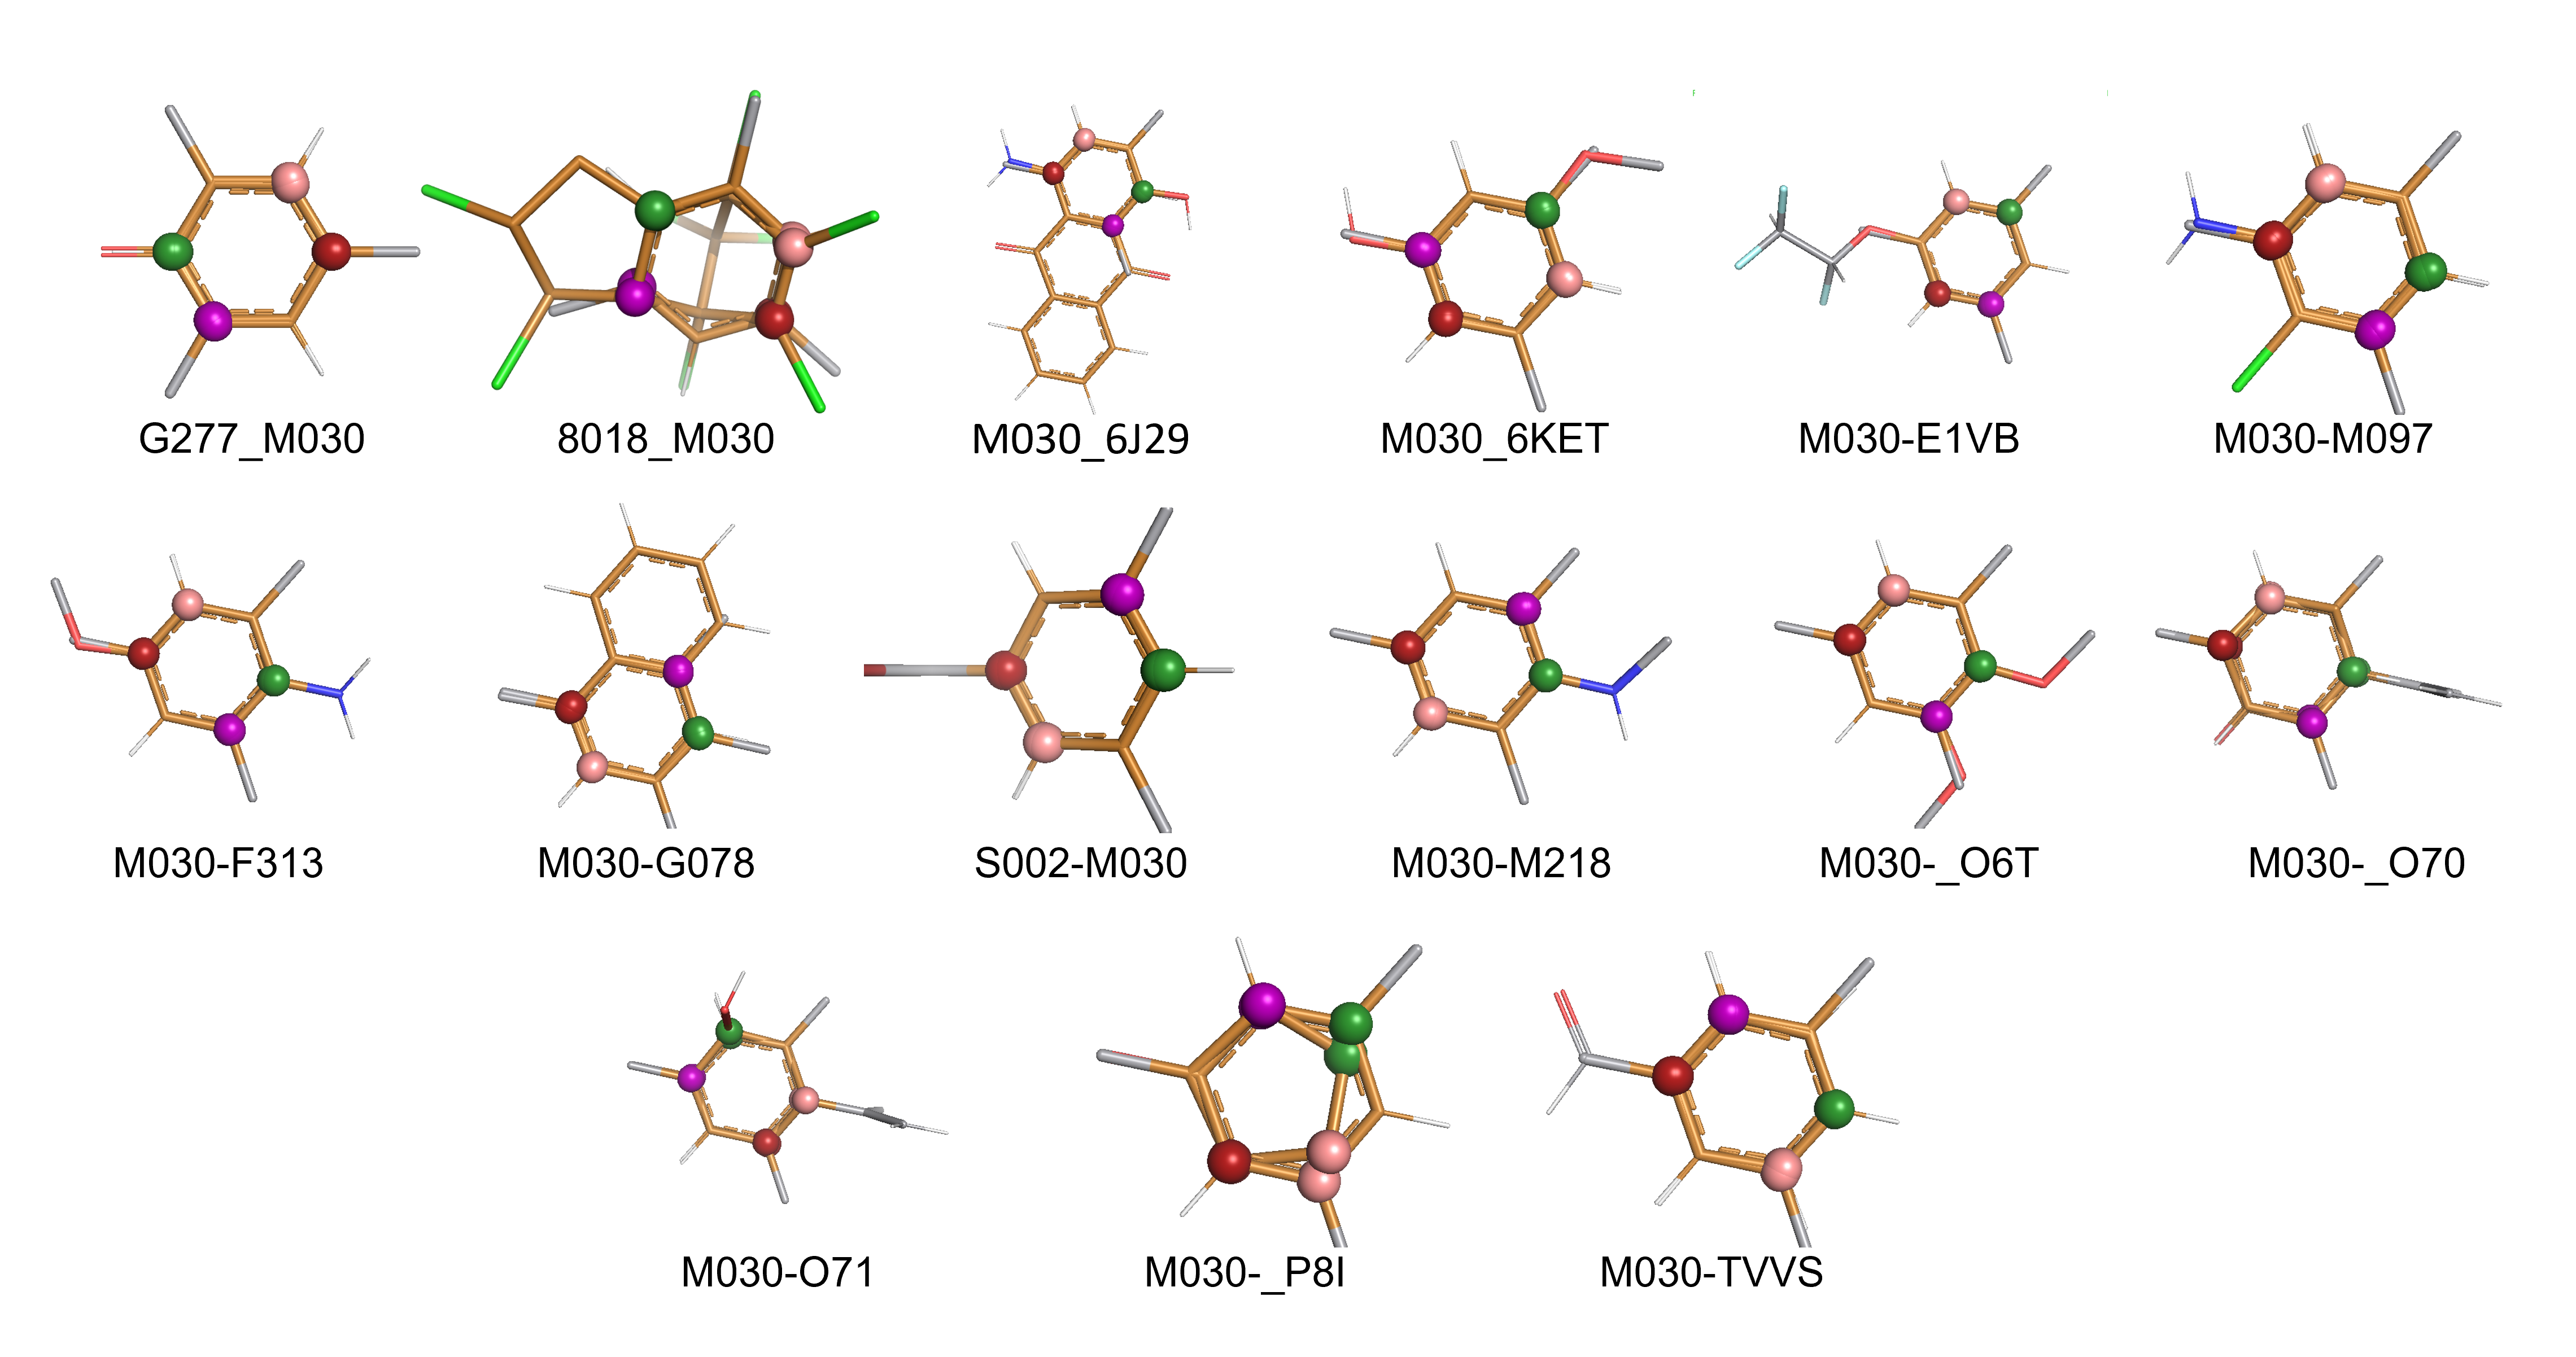
\includegraphics[width=\textwidth]{fig/results/pairwise/restraintPlacement/Restraints_PairwiseTI_M030Graph.png}
    \caption{Selected distance restraints (colored spheres) for the 15 pairwise TI calculations with molecule 12 (i.e. 1,3,5-timethylbenzene) as the central molecule (Figure \ref{fig: Pairwise_TI_M030_Graph}). For each pair, four distance restraints were determined with the greedy algorithm.}
    \label{SIfig: Pairwise_TI_M030_Graph}
\end{figure}


The computational boxes for the simulations in water were generated with the GROMOS++ \cite{Eichenberger2011} program \textit{simbox} using a minimal solute-to-wall distance of $0.8~$nm, and relaxed by energy minimization. The scripts can be found in the example folder on Github (\textit{https://github.com/rinikerlab/restraintmaker/tree/main/examples/\\publication/b\_ATB\_solvationFreeEnergies}).
The TI calculations were carried out with 21 evenly spaced $\lambda$-points between 0 and 1, both for the molecules in water and in vacuum. Each $\lambda$-point was equilibrated for $1$~ns, followed by a production run of $5$~ns. The free-energy differences were calculated using the Simpson integration implemented in the SciPy library.\cite{Virtanen2020}

\subsection{Analysis}
The analysis of the simulations was carried using GROMOS++ \cite{Eichenberger2011} and PyGromosTools \cite{Lehner2021}. In addition, the following Python packages were employed for the statistical analysis and plotting: Pandas \cite{Mckinney2010}, Matplotlib \cite{Hunter2007}, NumPy \cite{Vanderwalt2011}, SciPy \cite{Virtanen2020}, mpmath \cite{Johansson2013}, and Jupyter notebooks.\cite{Kluyver2016}


%================================================================================
\section{Results and Discussion}
%================================================================================

The chosen model system of five inhibitors of CHK1 kinase exemplifies different core-hopping transformations (i.e. ring size change, ring opening/closing, ring extension) and R-group modifications \cite{Wang2017}, increasing the complexity compared to the systems previously studied with RE-EDS. Furthermore, the performance can be directly compared to the results obtained with FEP+ and OPLS3 in Ref.~\cite{Wang2017} as well as with QligFEP results in Ref.~\cite{Jespers2019}.

\subsection{Parameter Exploration and Parameter Optimization}
The RE-EDS workflow was started by estimating the lower bound for the $s$-distribution. Using the above mentioned undersampling criterion (see Methods section), a lower bound of $s=0.01$ was determined for the protein-ligands complex and $s=0.0056$ for the ligands in water. 

%State Optimizations
Optimized coordinates were obtained for all five ligands, as verified by comparing the potential-energy distribution from the EDS simulation with the one extracted from a standard MD simulation of the respective ligand (Figure S1 in the Supporting Information). % SUPPL
From these same steps, the potential-energy thresholds for the occurrence sampling ($T_{i}^{\text{phys}}$) and undersampling ($T_{i}^{\text{us}}$) were estimated.

%Eoff:
The energy offsets $\vec{E}^R$ were estimated from a short RE-EDS simulation with the PEOE \cite{Sidler2016} scheme and are listed in Table \ref{tab:CHK1_set2_Eoff}.
For $s=1.0$, the energy offsets should ideally be equal to the free energy of the corresponding state (i.e. $\Delta E^R_{ji} = \Delta G_{ji}$) such that the partition function of the reference state is the sum of the partition functions of the end states \cite{Christ2008}. Therefore, the comparison between the relative estimated energy offsets in water and in complex ($\Delta \Delta E^R_{ji} = \Delta E^R_{ji,\text{complex}} - \Delta E^R_{ji,\text{water}}$) and the relative binding free energy $\Delta \Delta G^\text{bind}_{ji}$ can be used to (roughly) assess the quality of the estimated energy offsets. As shown in Figure S2 in the Supporting Information, % SUPPL
the energy offsets estimated from the SSM simulations are in better agreement with the experimental relative binding free energies than those estimated from the 1SS simulations.

\begin{table}[h]
\caption{Energy offsets $\vec{E^R}$ estimated from a short RE-EDS simulation using the PEOE \cite{Sidler2016} scheme. The errors indicate the standard deviation over the different replicas in undersampling. All energy offsets were calculated relative to ligand L1. The starting coordinates were selected following the 1SS or the SSM approach (see Theory and Methods sections).}
\label{tab:CHK1_set2_Eoff}
\resizebox{\columnwidth}{!}{%
\centering
\begin{tabular}{ l | r r | r r }
 Ligand & \multicolumn{2}{c|}{Water}&\multicolumn{2}{c}{Complex}  \\ 
  &RE-EDS 1SS [kJ~mol$^{-1}$]&RE-EDS SSM [kJ~mol$^{-1}$]&RE-EDS 1SS [kJ~mol$^{-1}$]&RE-EDS SSM [kJ~mol$^{-1}$]\\ 
 \hline
     L1 & $0.0$ & $0.0$ & $0.0$ & $0.0$ \\ 
     L17 & $11.07 \pm 7.61 $ & $17.81 \pm 0.69 $ & $20.03 \pm 5.04 $ & $18.19 \pm 3.43$ \\
     L19 & $-9.38 \pm 6.85 $ & $ -12.37 \pm 5.23 $ & $-2.09 \pm 1.56 $ & $ 2.4 \pm 1.56$ \\
     L20 & $-53.15 \pm 2.95 $ & $ -56.01 \pm 13.67 $ & $ -58.73 \pm 4.87 $ & $-52.2 \pm 2.6$\\
     L21 & $-76.75 \pm 5.79 $& $-69.15 \pm 3.74 $ & $ -77.29 \pm 3.12 $ & $ -77.9 \pm 3.4$\\
\end{tabular}
}
\end{table}

%S-Optimization
The optimization of the $s$-distribution was performed with the N-LRTO \cite{Sidler2017} algorithm, thereby minimizing the average round-trip time $\overline{\tau}$ in the replica graph. For the 1SS complex system, four optimization iterations were used. For the other systems, three iterations were used. 

%
In the first iteration, the total number of observed round trips was very low or zero for all approaches. In the following iterations, this quantity increased, and the average round-trip time decreased for all simulations (Figure \ref{fig: CHK1_RingOpening_sOptimization}). The number of round trips was generally smaller in the complex than in water due to a more pronounced gap region \cite{Sidler2017}.
Already after the second iteration, the round-trip time was reduced in all approaches, except for 
RE-EDS 1SS in the complex, where no round trips occurred during the second iteration. The improvement of the $\overline{\tau}$ over the iterations can also be seen in Figure S3 in the Supporting Information. % SUPPL
%% s-replica placements
As can be seen in the third row of Figure \ref{fig: CHK1_RingOpening_sOptimization}, the optimization algorithm increases the density of the replicas around $s = 0.041$, where the major gap region lies.

\begin{figure}[h]
\centering
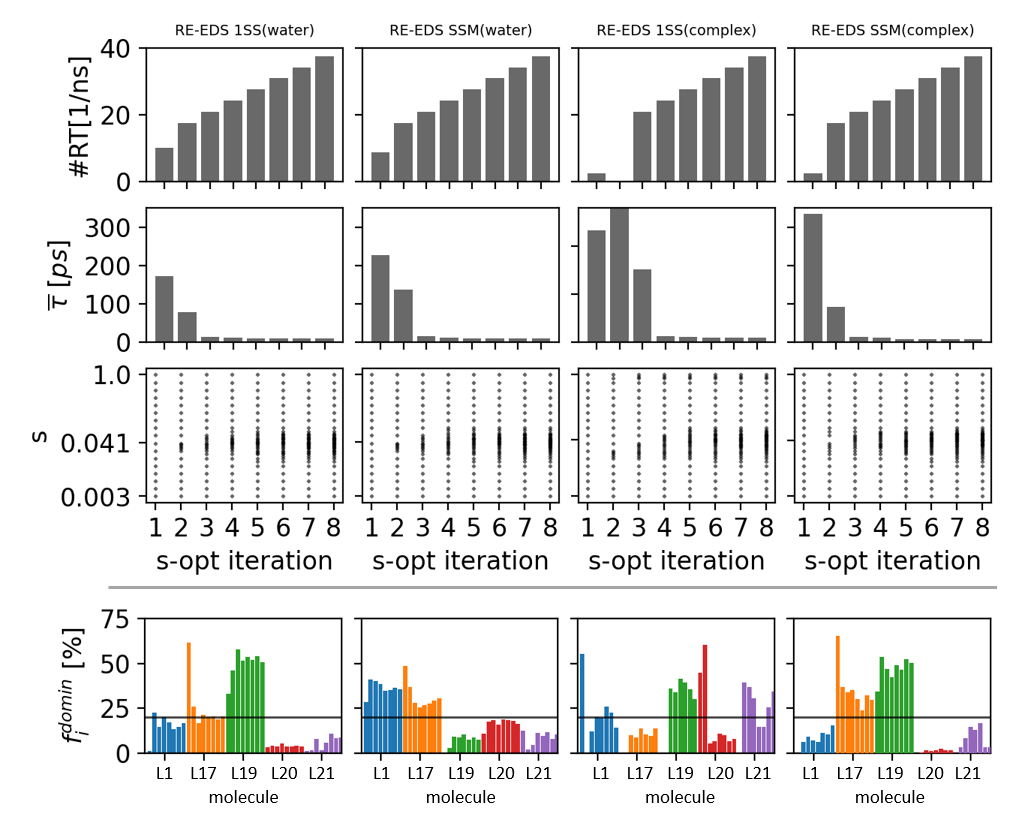
\includegraphics[width=\textwidth]{fig/results/ringOpening/paramOptimization/S-optimization_ringOpening.png}
\caption{Optimization steps of the $s$-distribution with the N-LRTO \cite{Sidler2017} algorithm followed by the energy offset rebalancing scheme (start indicated by the red horizontal line). The measured quality criteria were the number of round trips (1. row), the average round-trip time $\overline{\tau}$ (2. row), the placement of the replicas in $s$-space (3. row), and the sampling fractions of maximally contributing states $f_{i}^{\text{mc}}$ (4. row). The light colored bars of $f_{i}^{\text{mc}}$ indicate $s$-optimization iterations, whereas the fully colored bars indicate energy offset rebalancing steps. }
\label{fig: CHK1_RingOpening_sOptimization}
\end{figure}



%% tau converge - Conclusion
The $s$-optimization was stopped after a sufficiently high number of round trips and low round-trip time was reached. 
This resulted in 20 replicas for the ligands in water after three $s$-optimization iterations.
For the protein-ligands complex, the fourth $s$-optimization iteration was chosen for the 1SS approach, and the third iteration for the SSM approach, resulting in 29 and 25 replicas, respectively. 
The average round-trip time after convergence was $\overline{\tau} = 0.4 \pm 0.2$~ns for all simulations.

After the $s$-optimization, the energy offset rebalancing scheme was applied to improve the state sampling. 

%RT analysis
During the rebalancing steps, no further replicas were added to the $s$-distribution. It is essential for the success of the rebalancing scheme that round trips occur. Therefore, the number of round trips and average round-trip time were monitored. In all systems, the number of round trips and $\overline{\tau}$ remained relatively stable over the four rebalancing steps. For the RE-EDS 1SS approach in water, the number of round trips slightly decreased but never dropped to zero.

%% states sampling
Across the optimization steps, also the sampling of the end states as maximally contributing states at $s=1.0$ was monitored.
During the $s$-optimization, some end states ``vanish'' and are no longer sampled as maximal contributing states. This leakage effect can occur when the initially estimated $E^{\text{R}}$ are not exactly optimal \cite{Sidler2016}. 
With energy offset rebalancing, the sampling of each end state can be recovered, and the sampling distribution is approaching the ideal case.
%After the s-optimization the MAE($P^{\text{maxContrib}}$) was for all approaches approximately at $25\%$, with the exception of the 1SS water system, here it was $20\%$. 
After rebalancing, all end states showed a $f_i^{\text{mc}} > 0$ and the mean absolute deviation of the sampling distribution from ideal decreased from $20-25\%$ to approximately $7-12\%$ (Figure S4 in the Supporting Information). % SUPPL
 
\subsection{Free-Energy Calculation}
After successfully optimizing the RE-EDS parameters, the production runs were performed for $3.5$~ns. 

%%Sampling++
Both in water and in complex, the potential-energy distributions of the end states generally match well the corresponding distributions from the standard MD simulations of the single end states (Figure \ref{fig:RingOpening_sampling_comparison}). Only in the complex 1SS approach, a deviation can be seen for L17, with a slight shift to higher potential energies. This is due to insufficient sampling of L17 in this case (see below). 
%
The analysis of the maximally contributing end states at $s=1.0$ shows that in water all end states were sampled close to the ideal equal distribution (Figure S5 in the Supporting Information). % SUPPL
In the simulation of the protein-ligands complex, there are still differences in sampling. Especially with the 1SS approach, L19 is generally sampled too much, while L17 is not sampled enough. The situation is improved with the SSM approach.
Comparing $f_i^{\text{occur}}$ and $f_i^{\text{mc}}$ in Figure S5 indicates that the end states in the CHK1 system are clearly separated (i.e. no phase-space overlap). % SUPPL

\begin{figure}[h]
    \centering
    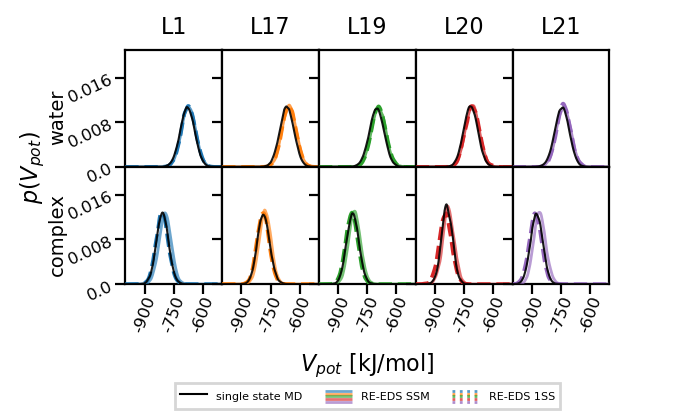
\includegraphics[width=\columnwidth]{fig/results/ringOpening/FE/RingClosure_system_final_sampling.png}
    \caption{Comparison of the Boltzmann reweighted potential-energy distributions obtained from standard MD simulations of a given end state (black) and from the RE-EDS production runs of the 1SS (green) and SSM (turquoise, dashed) approaches.}
    \label{fig:RingOpening_sampling_comparison}
\end{figure}

%%Accuracy
From the replica at $s=1.0$, the free-energy differences were calculated using Eq.~(\ref{EQ: Free Energy calculation via reference state}) and the resulting $\Delta \Delta G^\text{bind}_{ji}$ were compared with the experimental results taken from Ref.~\cite{Huang2012}. The results are shown graphically in Figure \ref{fig:CHK1_set2_FreeEnergyCalculation} and numerically in Table \ref{tab: RE-EDS_FE_RingCycleOpening_ddF}. The individual free-energy differences are given in Table S3 in the Supporting Information. %SUPPL
The RMSE with RE-EDS 1SS is $4.4$~kJ~mol$^{-1}$ and the MAE is $3.9\pm2.8$~kJ~mol$^{-1}$. 
%
%how I calculate the MAE and RMSD:
%MAE = np.mean(np.abs(ddG_differences))
%std(MAE) = np.std(np.abs(ddG_differences)) #gives an impression of absolute deviation of all ddG_diffs
%RMSE = np.sqrt(np.mean(np.square(ddG_differences))
%
The main deviations stem from ligand L17 in the RE-EDS 1SS approach, which can be explained by the insufficient sampling of L17 in the complex (see Figure \ref{fig:RingOpening_sampling_comparison} and Figure S5 in the Supporting Information). %SUPPL

The performance was substantially improved using the SSM approach with RE-EDS, giving an RMSE of $3.3$~kJ~mol$^{-1}$ and an MAE of $2.8 \pm 1.7$~kJ~mol$^{-1}$. 
Only two values (L21-L11) and (L21-L19) deviate more than $4.184$~kJ~mol$^{-1}$ (i.e. $1$~kcal~mol$^{-1}$) from experiment.
The Spearman correlation coefficient for RE-EDS 1SS is $r^2_{\text{Spearman}}=0.01$ and for RE-EDS SSM $r^2_{\text{Spearman}}=0.69$.

%%Performance:
Next, we assessed the convergence of the $\Delta G_{ji}$ values as a function of simulation time (Figure S6 in the Supporting Information). % SUPPL
For the RE-EDS 1SS approach, all free-energy differences appeared converged after $2.5$~ns in water and after $2.7$~ns in the complex. For the RE-EDS SSM approach, convergence was observed after $2.5$~ns in water and after $2.9$~ns in the complex.

\begin{figure}[h]
    \centering
    \begin{subfigure}{0.85\columnwidth}
        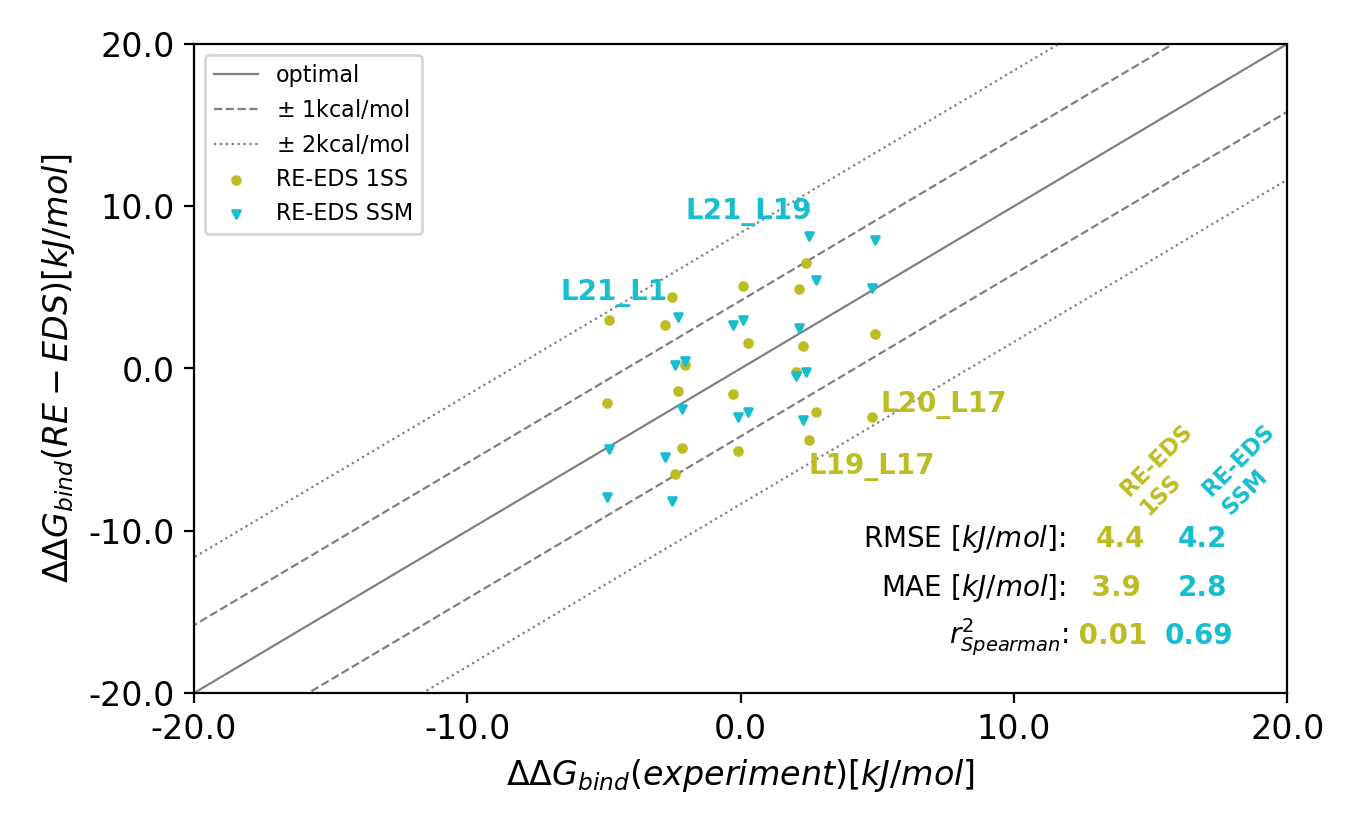
\includegraphics[width=\textwidth]{fig/results/ringOpening/FE/RingClosure_system_final_results_4ns_comparison.png}
        \end{subfigure}
    \begin{subfigure}{0.85\columnwidth}
        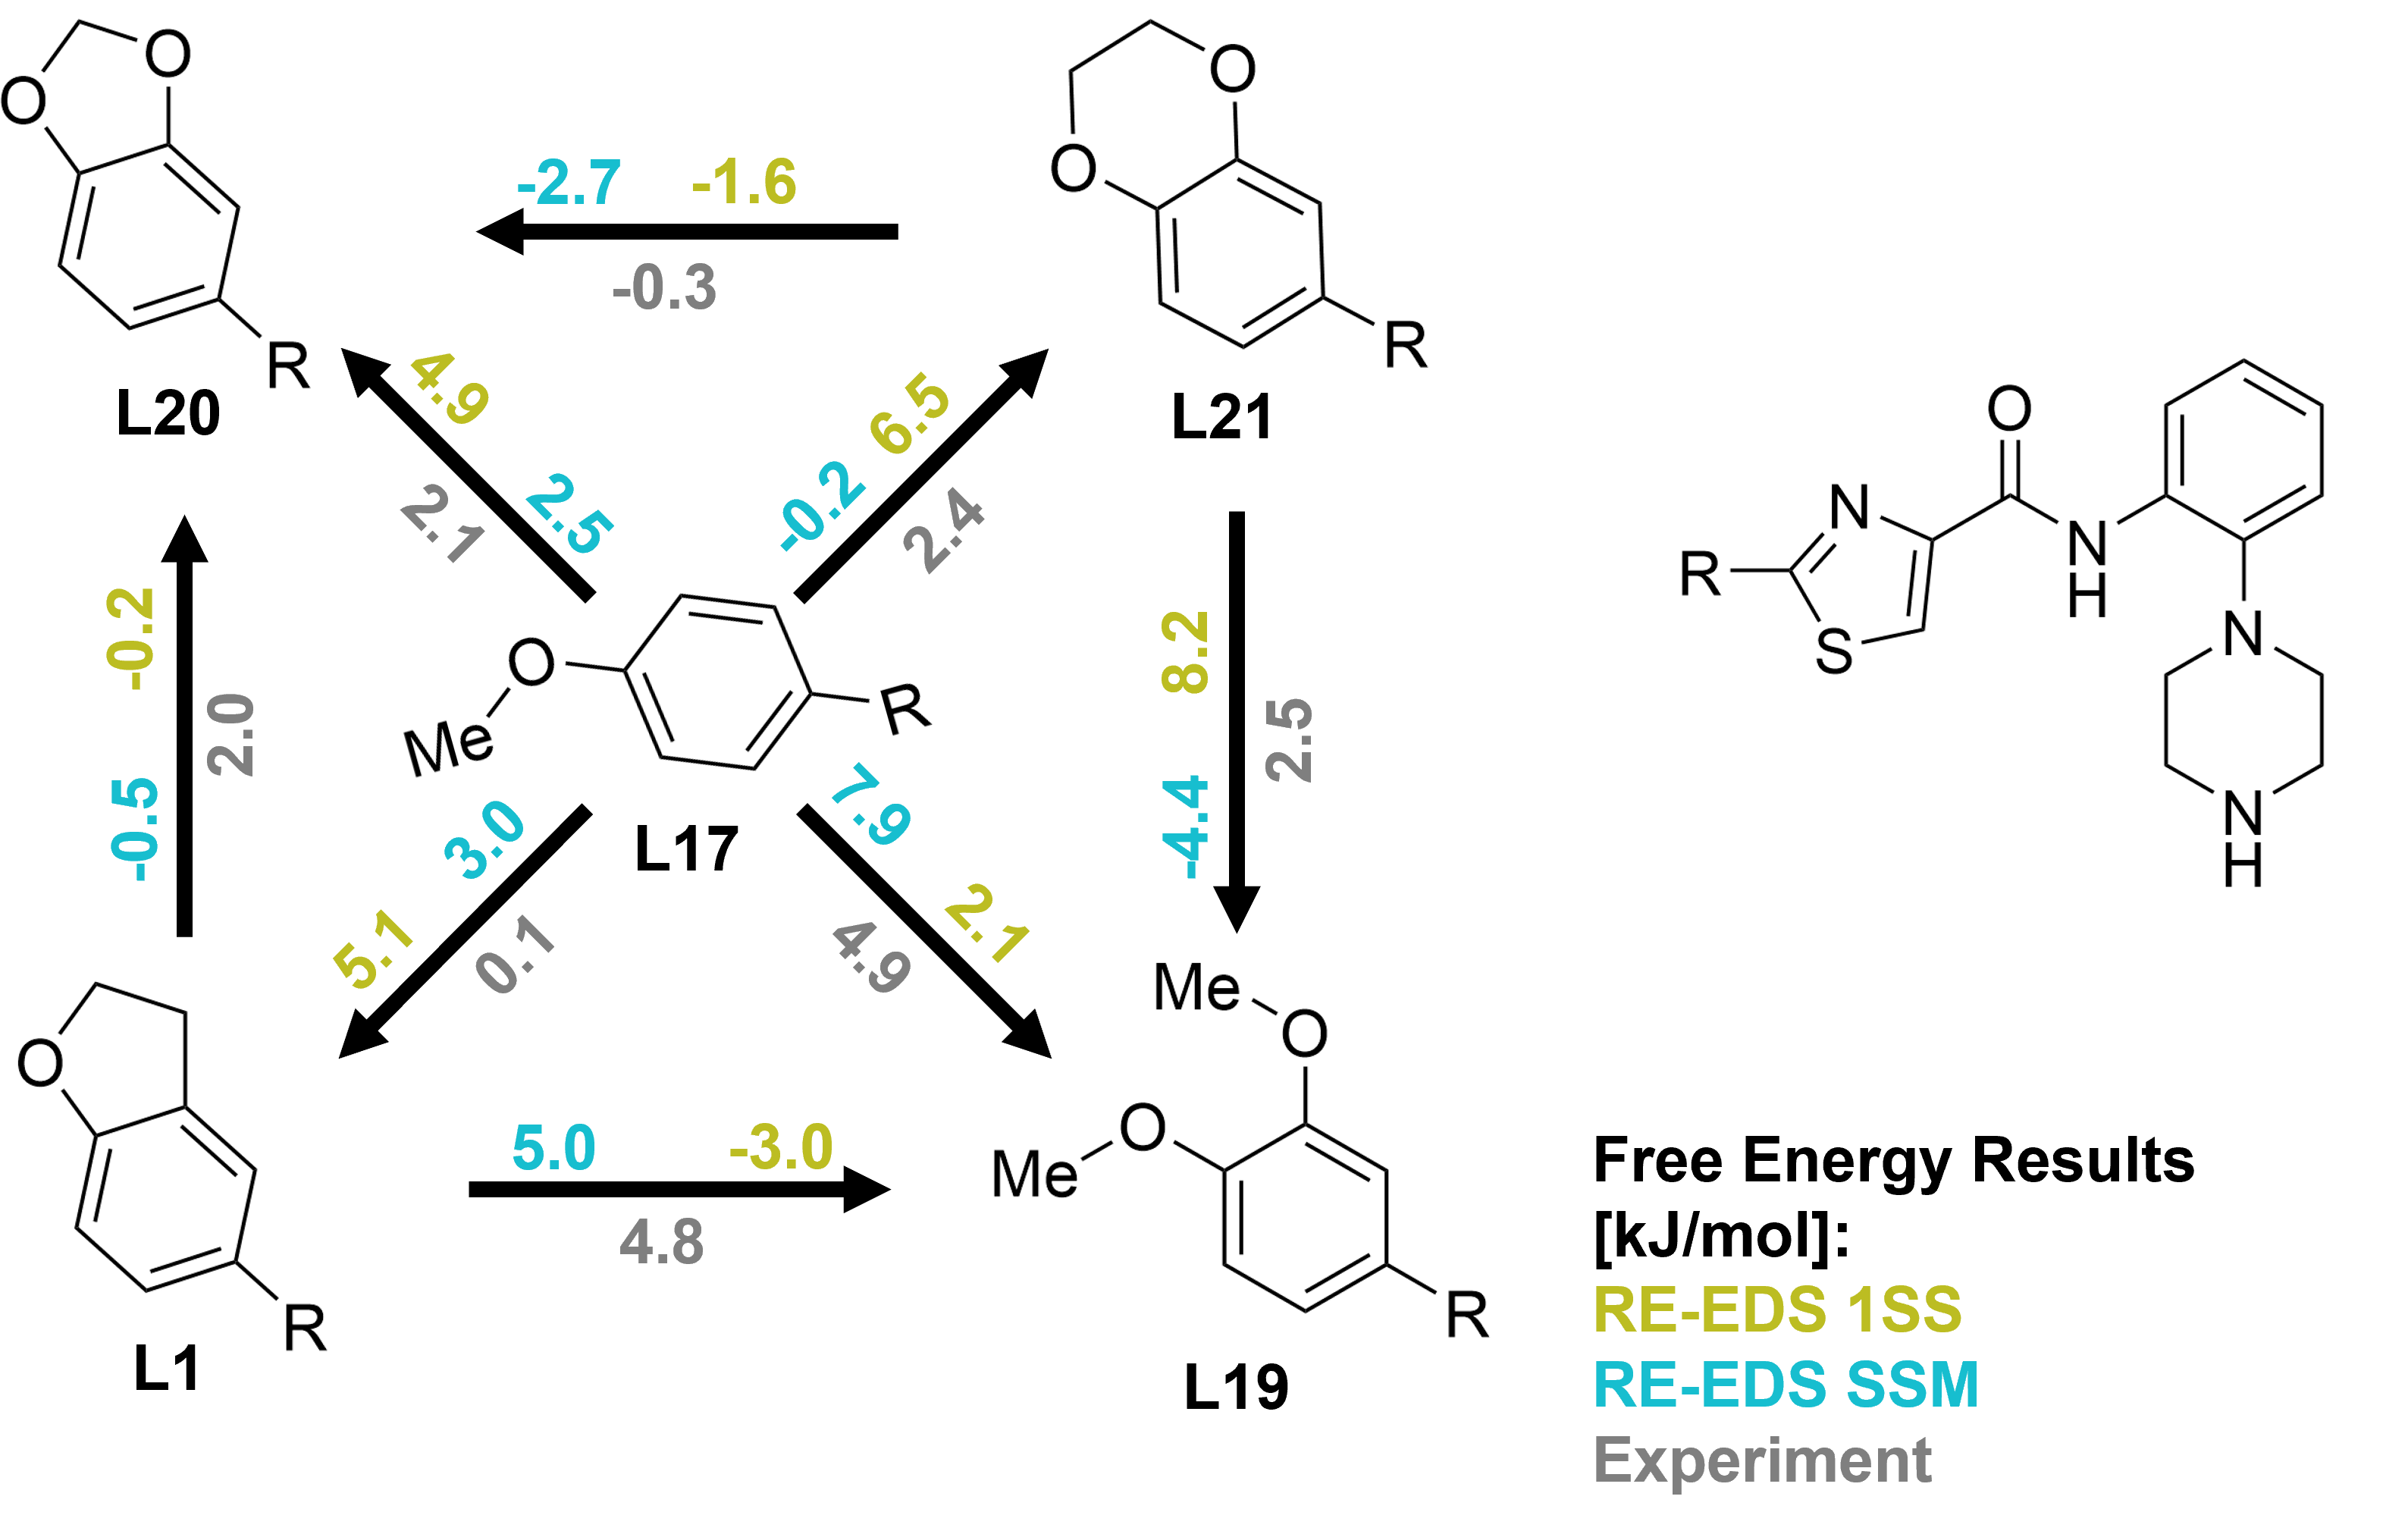
\includegraphics[width=\textwidth]{fig/results/ringOpening/FE/ddG_bind_paper_comparison_reeds_only_4nsSimulation.png}
        \end{subfigure}
    \caption{Free-energy differences estimated from the production run of $3.5$~ns length. (Top): Comparison between the experimental and calculated $\Delta \Delta G^\text{bind}_{ji}$ using RE-EDS 1SS and RE-EDS SSM. The results were calculated with all possible pairwise transformations (forward and backward). (Bottom): Graphical representation of the $\Delta \Delta G^\text{bind}_{ji}$ results with structures, inspired by the one in Ref.~\cite{Wang2017}.}
    \label{fig:CHK1_set2_FreeEnergyCalculation}
\end{figure}

%Comparison results with Schroedinger & Jespers
By applying the RE-EDS methodology to the same system of five CHK1 inhibitors as studied by Wang \textit{et. al.} \cite{Wang2017} and later on also Jespers \textit{et al.} \cite{Jespers2019}, a direct comparison with FEP+ and QligFEP is possible (Table \ref{tab: RE-EDS_FE_RingCycleOpening_ddF}). Note that the quality metrics were calculated over all possible pairs of ligands and in both directions, not only those directly calculated by FEP+ and QligFEP.
For FEP+, we obtained an RMSE of $2.4$~kJ~mol$^{-1}$ and an MAE of $1.8 \pm 1.2$~kJ~mol$^{-1}$ with a Spearman correlation coefficient of $r^2_{\text{Spearman}}=0.67$.
Including cycle closure correction (CC) \cite{Wang2017} reduced the RMSE to $2.1$~kJ~mol$^{-1}$ and the MAE to $1.9 \pm 1.0$~kJ~mol$^{-1}$. The Spearman correlation coefficient increased to $r^2_{\text{Spearman}}=0.73$.
Jespers \textit{et al.} \cite{Jespers2019} reported free-energy differences with QligFEP as an average over ten independent replicas, each with significantly less simulation time per $\lambda$-window than in Ref.~\cite{Wang2017}. For QligFEP, an RMSE of $2.3$~kJ~mol$^{-1}$, an MAE of $2.0 \pm 1.2$~kJ~mol$^{-1}$, and a Spearman coefficient of $r^2_{\text{Spearman}}=0.61$ was obtained.

Overall, the performance of RE-EDS SSM is comparable with the pairwise methods. The results with FEP+ CC and QligFEP showed a slightly higher accuracy compared to experiment, likely due to the different force fields used. The Spearman correlation coefficient is comparable with the other methods for the RE-EDS SSM approach.

\begin{table}[h]
\caption{Relative binding free energies $\Delta \Delta G^\text{bind}_{ji}$ from experiment and calculated with the RE-EDS 1SS and RE-EDS SSM approaches. For comparison, the results for FEP+ with and without cycle closure (CC) correction taken from Ref.~\cite{Wang2017} and the results for QligFEP taken from Ref.~\cite{Jespers2019} are listed. The free-energy differences of directly simulated paths were used to infer not directly simulated free-energy differences (marked in bold). If multiple indirect paths were possible, their average was used. The errors for QligFEP were determined in Ref.~\cite{Jespers2019} by calculating the standard deviation over ten replicas. For FEP+, the error of the results was taken from the used BAR \cite{Bennett1976} method and the FEP+ CC errors were obtained from the cycle closure analysis. For the RE-EDS approaches, the reported error is based on the statistical uncertainties of the $\Delta G_{ji}^{env}$ values estimated using Gaussian error approximation \cite{Christ2008}. The uncertainty estimate of the RMSE was obtained by a 100-fold bootstrapping approach. }
\begin{center}
\footnotesize
\resizebox{\columnwidth}{!}{%
\begin{tabular}{ c c |c |c|c|c|c|c}
  \multicolumn{2}{c|}{Ligands} & \multicolumn{1}{c|}{Exp. \cite{Huang2012}} &\multicolumn{1}{c|}{FEP+ \cite{Wang2017}}&\multicolumn{1}{c|}{FEP+ CC \cite{Wang2017}}&\multicolumn{1}{c|}{QligFEP \cite{Jespers2019}}&\multicolumn{1}{c|}{RE-EDS 1SS}&\multicolumn{1}{c}{RE-EDS SSM}\\ 
    $i$ & $j$  & [kJ~mol$^{-1}$]  & [kJ~mol$^{-1}$] & [kJ~mol$^{-1}$] & [kJ~mol$^{-1}$] & [kJ~mol$^{-1}$] & [kJ~mol$^{-1}$]  \\
  \hline
        L17 &  L1 &   0.1 & -3.6 $\pm$ 0.4          & -2.9 $\pm$ 1.0         & -1.6 $\pm$ 1.7                                     &    5.1 $\pm$ 0.8 &  3.0 $\pm$ 2.0 \\
        L19 &  L1 &  -4.8 & -3.9 $\pm$ 0.3          & -4.0 $\pm$ 0.6         & -1.7 $\pm$ 2.0                                     &    3.0 $\pm$ 1.0 & -5.0 $\pm$ 0.1\\
        L20 &  L1 &  -2.0 & -2.5 $\pm$ 0.1          & -3.1 $\pm$ 1.0         & -1.3 $\pm$ 1.3                                     &    0.2 $\pm$ 0.9 &  0.5 $\pm$ 0.1\\
        L21 &  L1 &  -2.3 &\textbf{-3.4} $\pm$ \textbf{0.7}  &\textbf{-3.2} $\pm$ \textbf{1.3} & \textbf{-0.1} $\pm$ \textbf{3.5} &   -1.4 $\pm$ 0.8 &  3.2 $\pm$ 0.1\\
        L19 &  L17 & -4.9 & -1.4 $\pm$ 0.3          & -1.1 $\pm$ 1.0         & \textbf{0.1} $\pm$ \textbf{2.6}                    &   -2.1 $\pm$ 0.6 & -7.9 $\pm$ 1.9\\
        L20 &  L17 & -2.1 &  0.3 $\pm$ 0.4          & -0.1 $\pm$ 0.8         & -1.3 $\pm$ 2.3                                     &   -4.9 $\pm$ 0.1 & -2.5 $\pm$ 1.9\\
        L21 &  L17 & -2.4 & -1.1 $\pm$ 0.4          & -0.9 $\pm$ 0.9         &\textbf{0.7} $\pm$ \textbf{2.6}                     &  -6.5 $\pm$ 0.1 &  0.2 $\pm$ 1.9\\
        L20 &  L19 & 2.8  &\textbf{0.8} $\pm$ \textbf{0.6}   & \textbf{0.1} $\pm$ \textbf{1.3} & \textbf{-0.4} $\pm$ \textbf{3.7} &  -2.7 $\pm$ 0.6 &  5.4 $\pm$ 0.1\\
        L21 &  L19 & 2.5  & -0.1 $\pm$ 0.6         &  0.6 $\pm$ 0.1         &  0.6 $\pm$ 4.9                                      &  -4.4 $\pm$ 0.6 &  8.2 $\pm$ 0.1\\
        L21 &  L20 & -0.3 & -0.3 $\pm$ 0.8         & -0.6 $\pm$ 0.8         &  0.6 $\pm$ 1.1                                    &    -1.6 $\pm$ 0.1 &   -2.7 $\pm$ 0.1\\ 
    \hline
        \multicolumn{2}{c|}{RMSE} &                    & 2.4  $\pm$ 0.3           & 2.1  $\pm$ 0.2          &  2.3  $\pm$ 0.38      & 4.4 $\pm$ 0.5         & 3.3  $\pm$ 0.3 \\
        \multicolumn{2}{c|}{MAE} &                     & 1.8 $\pm$ 1.2 & 1.9 $\pm$ 1.0 & 2.0 $\pm$ 1.2 & 3.9 $\pm$2.8 & 2.8 $\pm$ 1.7 \\
        %\multicolumn{2}{c|}{$r^2_{\text{Pearson}}$} & & 0.66            & 0.67          & 0.63          & -0.07m          & 0.71 \\
        \multicolumn{2}{c|}{$r^2_{\text{Spearman}}$} & & 0.67           & 0.73          & 0.61          & 0.01           & 0.69 \\
        \multicolumn{2}{c|}{$t_{simulation} [ns]$} & & 640          &  640         &  51        & 171.5         & 157.5  \\
\end{tabular}
}
\end{center}
\label{tab: RE-EDS_FE_RingCycleOpening_ddF}
\end{table}

% 
%FEP+: 
%MAE 1.99 +- 1.4
%RMSE 2.43
%r^2 pearson 0.56 	 r^2 spearman 0.56
%
%FEP+ CC: 
%MAE 1.88 +- 1.05
%RMSE 2.15
%r^2 pearson 0.66 	 r^2 spearman 0.71

%QLigFEP
%MAE 1.97 +- 1.2
%RMSE 2.3
%r^2 pearson 0.63 	 r^2 spearman 0.61


%ComputationalCost
%FEP: 16 l-windwos*5ns*4 pairs * 2 approaches ==> 640ns
%QligFEP: 10 repetitions * (eq 131ps + 51lams * 10ps sim) * 4 pairs * 2 approaches ==> 51ns
%Complex: 
%	- Optimization: 1ns * 17 Eoff + 0.5ns*17 sopt1 + 1ns*21 sopt2 + 3*0.5ns*25 eoffRB = 84ns
%	- Production: 25*3.5 = 87.5ns / 29*3.5 =  101.5
%Water:
%	- Optimization: 1ns * 12 Eoff + 0.5ns*12 sopt1 + 1ns*16 sopt2 + 3*0.5ns*20 eoffRB = 64ns
%   - Production: 20 * 3.5maybe = 70ns
%old reeds line complex - optim: eoff(21*0.8)+sop1(0.4ns*21)+sopt2(0.8ns*25)+sopt3(1.2ns*29)+sopt4(1.2ns*31)+sopt5(1.2ns*35) = 276.4 ns
%old reeds line complex - prod: 4ns*41 = 164 ns
%new reeds line complex - optim: eoff(21*0.8)+sop1(0.4ns*21)+sopt2(0.8ns*25)+sopt3(1.2ns*29)+eoffRB(0.5ns*2*29) = 122 ns
%new reeds line complex - prod: 4ns*29 = 116ns 

In terms of computational cost, the RE-EDS approach (with $3.5$~ns per replica) resulted in about a quarter of the total simulation time (in ns) than reported for the FEP+ calculations in Ref.~\cite{Wang2017} (Table \ref{tab: RE-EDS_FE_RingCycleOpening_ddF}). However the QligFEP approach is the approach with the lowest simulation time consumption. A major advantage of the simultaneous simulation of multiple ligands in a single RE-EDS simulation is that all $N(N-1)/2$ transformations are sampled directly, leading to low statistical errors and removing the need of a state graph. This advantage increases with increasing number of ligands. The current workflow of RE-EDS uses a relatively large amount of simulation time for parameter optimization. Future work will focus on further optimization of the workflow to reduce the pre-processing time. 

From the calculated relative binding free energies, $\Delta G_{i}^{\text{bind}}$ can be obtained by using one experimental value as anchor point. This allows us to generate a ranking of the five ligands. To avoid any bias from the selected experimental anchor point, all possibilities were calculated and the resulting values averaged (Table \ref{tab:RE-EDS_FE_RingCycleOpening_absoluteShiftDF}). While the RMSE is generally low for all approaches ($<$ 1 kcal mol$^{-1}$ = 4.184 kJ mol$^{-1}$), the ranking of the ligands as measured by $r^2_{\text{Spearman}}$ is not very good. 
%A strong correlation with experiment is of interest in drug design approaches, as the ranking of ligands in virtual screening is important to suggest the most promising drug candidates to be synthesized.
This observation is not uncommon for ligand series with small differences in binding free energy \cite{wang2015,schindler2020}.
Note that the uncertainties of the individual values have increased compared to the relative binding free energies due to the anchoring and averaging procedure.

\begin{table}[h]
\caption{Absolute binding free energies $\Delta G_{i}^{\text{bind}}$ and ranking of the ligands derived from the relative binding free energies. The values were calculated from the relative binding free energies using an experimental binding free energy as anchor point, and then averaged over the five possibilities. The errors are standard deviations over the possible outcomes. For comparison, the results for FEP+ with and without cycle closure (CC) correction taken from Ref.~\cite{Wang2017} and the results for QligFEP taken from Ref.~\cite{Jespers2019} are shown (calculated with the same procedure). The uncertainty estimate of the RMSE was obtained by a 100-fold bootstrapping approach.}
\begin{center}
\footnotesize
\resizebox{\columnwidth}{!}{%
\begin{tabular}{ c |c |c|c|c|c|c}
  Ligands & \multicolumn{1}{c|}{Exp. \cite{Huang2012}} &\multicolumn{1}{c|}{FEP+ \cite{Wang2017}}&\multicolumn{1}{c|}{FEP+ CC \cite{Wang2017}}&\multicolumn{1}{c|}{QligFEP \cite{Jespers2019}}&\multicolumn{1}{c|}{RE-EDS 1SS}&\multicolumn{1}{c}{RE-EDS SSM}\\ 
    Molecule & [kJ~mol$^{-1}$]  & [kJ~mol$^{-1}$] & [kJ~mol$^{-1}$] & [kJ~mol$^{-1}$] & [kJ~mol$^{-1}$] & [kJ~mol$^{-1}$]  \\
  \hline
        L1 &   -40.7 & -41.7 $\pm$ 1.7         & -41.7 $\pm$ 0.9         & -38.5 $\pm$ 1.5 &   -40.0 $\pm$ 3.4 &    -38.0 $\pm$ 2.0 \\
        L17 &  -40.8 &  -38.0 $\pm$ 1.0         & -38.2 $\pm$ 1.1         & -38.6 $\pm$ 1.3 &    -33.7 $\pm$ 1.3 & -41.7 $\pm$ 2.3 \\
        L19 &  -35.9  & -38.1 $\pm$ 0.9         & -38.3 $\pm$ 1.8         & -38.3 $\pm$ 1.0 &   -37.6 $\pm$ 3.3 &  -33.0 $\pm$ 2.0 \\
        L20 &  -38.6 & -38.6  $\pm$ 1.6         & -38.3 $\pm$ 1.4         & -39.2 $\pm$ 1.7 &    -40.4 $\pm$ 3.3 & -39.1 $\pm$ 2.3 \\
        L21 &  -38.4 & -37.7  $\pm$ 1.4         & -37.8 $\pm$ 1.3         & -39.4 $\pm$ 1.9 &    -42.4 $\pm$ 2.9 &    -42.5 $\pm$ 1.4 \\
    \hline
        RMSE &                    & 1.7  $\pm$  0.4        & 1.7   $\pm$ 0.4        & 1.7 $\pm$ 0.4          & 3.8 $\pm$ 1.3         & 2.6 $\pm$ 0.6 \\
        MAE &                     & 1.3 $\pm$ 1.0  & 1.4 $\pm$ 0.9 & 1.4 $\pm$ 0.9 & 3.0 $\pm$ 2.3 & 2.2 $\pm$ 1.6 \\
        $r^2_{\text{Spearman}}$ &  & 0.20           & 0.10          & -0.21         &  -0.40           & 0.30 \\
\end{tabular}
}
\end{center}
\label{tab:RE-EDS_FE_RingCycleOpening_absoluteShiftDF}
\end{table}


\section{Parameter Exploration}
A fast transition of the initial maximally contributing end state to the desired maximally contributing end state was observed by monitoring the maximally contributing end state over time.
The transition occurred latest after $0.5$~ns, and the system remained in the biased end state for the rest of the simulation time.
In both water and complex simulations, the desired end state was sampled about $~99\%$ of the simulation time with the exception of L19 in water (Table \ref{SItab:RingCycleOpenin_sampling_fraction_optimizedStates}).
To inspect if the optimized state simulations' results sufficiently represent the target states, a comparison between the target state obtained potential-energy distributions in the EDS simulations with MD simulations consisting of only the target state was conducted (Figure \ref{fig:CHK1_set2_stateOptimization_EnergyDistribution}). 

\begin{table}[H]
\centering
\caption{Fraction of the simulation time $f_i^{\text{mc}}$ (in \%) that the desired end state was sampled as the maximally contributing state during the EDS simulation to optimize the coordinates for a desired end state.}
\label{SItab:RingCycleOpenin_sampling_fraction_optimizedStates}
\begin{tabular}{ l | c c }
 Ligand & Water  & Complex \\ 
 \hline
     L1 & 99.84 & 99.97 \\ 
     L17 & 99.99 & 99.97\\
     L19 & 36.07 &  99.98\\
     L20 & 99.99 & 100\\
     L21 & 100 & 99.97 \\
\end{tabular}
\end{table}

\begin{table}[H]
\centering
\caption{Potential thresholds for occurrence sampling ($T_{i}^{\text{phys}}$) and undersampling ($T_{i}^{\text{us}}$) determined during the parameter exploration (in kJ~mol$^{-1}$).}
\label{SItab:RingCycleOpenin_PotentialTresholds}
\begin{tabular}{ l | c c |c c| }
 Ligand &\multicolumn{2}{c|}{Water} & \multicolumn{2}{c|}{Complex}\\ 
  & \multicolumn{1}{c}{$T^{\text{phys}}$}& \multicolumn{1}{c|}{$T^{\text{us}}$}&  \multicolumn{1}{c}{$T^{\text{phys}}$}& \multicolumn{1}{c|}{$T^{\text{us}}$} \\ 
 \hline
     L1  & -582.96 & -436.05 & -737.37 & -516.41\\ 
     L17 & -572.41 & -419.16 & -717.95 & -492.83\\
     L19 & -579.13 & -415.91 & -738.95 & -483.78\\
     L20 & -636.00 & -492.75 & -759.01 & -549.35\\
     L21 & -656.22 & -488.43 & -805.30 & -539.78\\
\end{tabular}
\end{table}

\begin{figure}[H]
\centering
     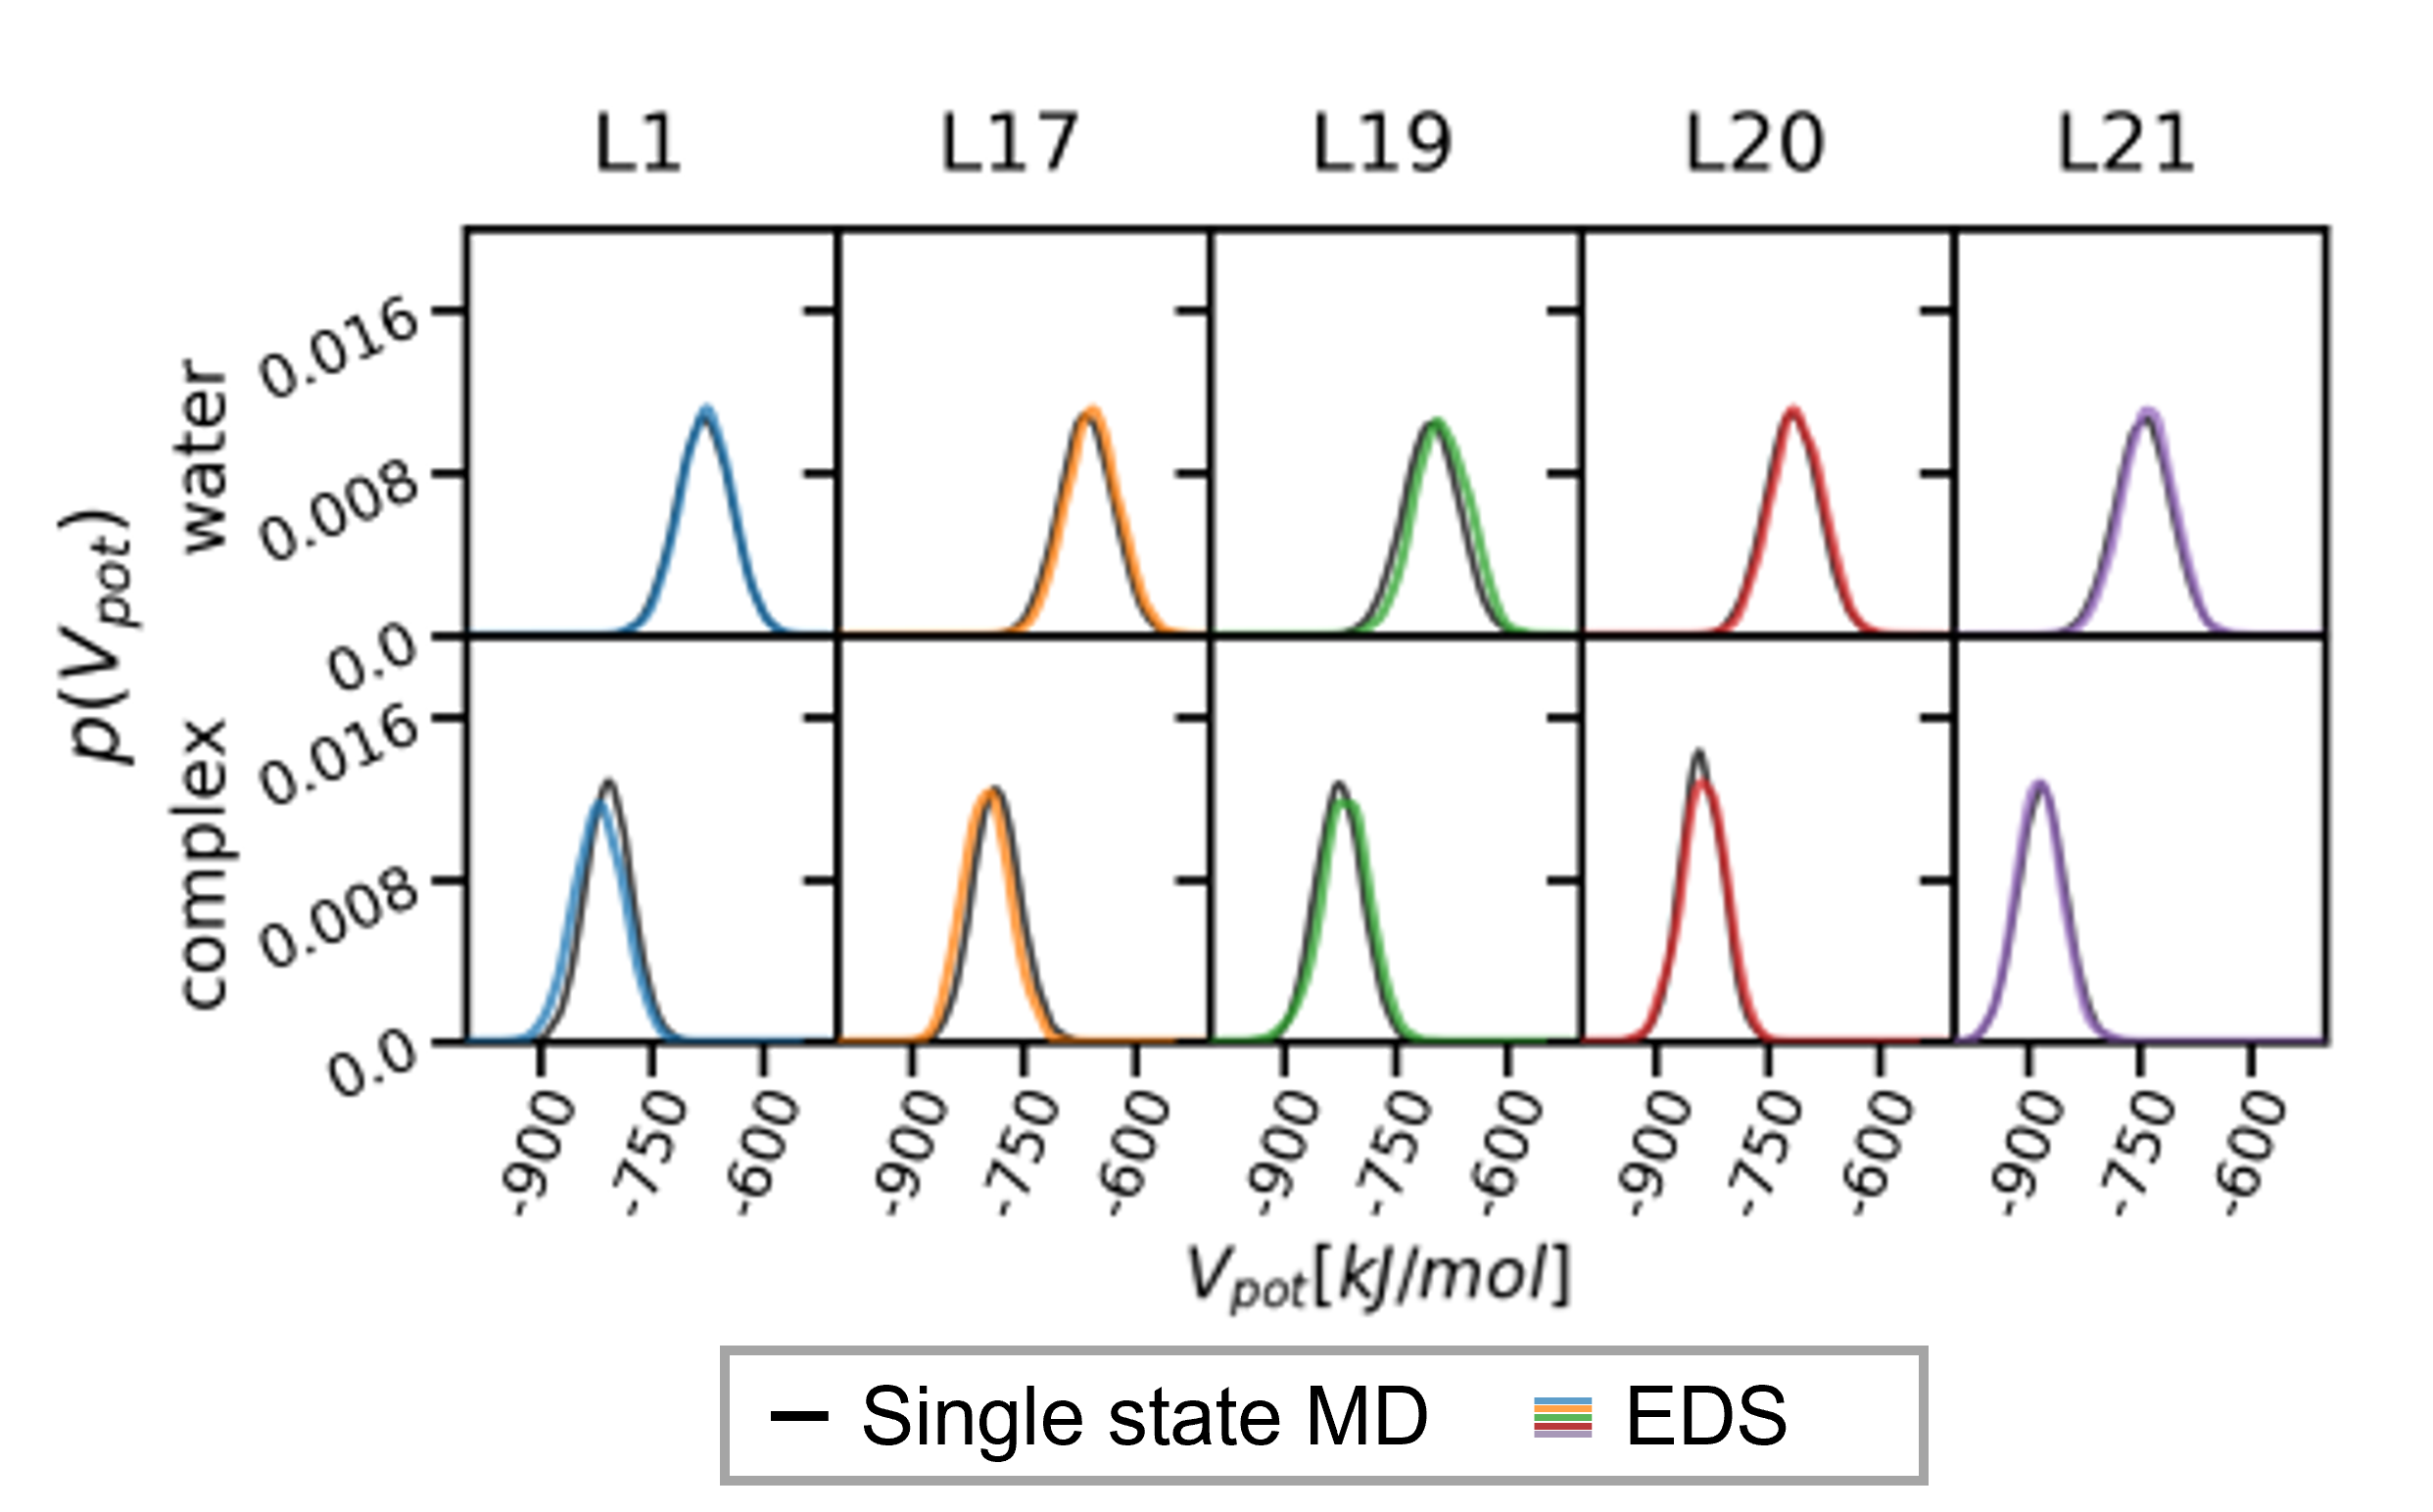
\includegraphics[width=0.8\textwidth]{fig/results/ringOpening/paramExploration/single_state_energy_sampling.png}
    \caption{Comparison of the potential-energy distribution obtained from a standard MD simulation of a given end state (black) and from an EDS simulation with the given end state favoured (colored) from the first step of the RE-EDS workflow.}
     \label{fig:CHK1_set2_stateOptimization_EnergyDistribution}
\end{figure}

\newpage
\section{Energy Offset Estimation}
The relative energy offsets $\Delta \Delta E^R_{ji}$ are compared with the experimental relative binding free energies $\Delta \Delta G^\text{bind}_{ji}$ in Figure \ref{SIfig:Eoff_experiment_corr_RingOpening}. 
The root mean squared error (RMSE) between $\Delta \Delta E^R_{ji}$ obtained with RE-EDS 1SS and $\Delta \Delta G^\text{bind}_{ji}$ is $12.6$~kJ~mol$^{-1}$. Outliers are mainly related to L19.
With the RE-EDS SSM approach, the RMSE was reduced to $7.0$~kJ~mol$^{-1}$. No clear outliers were observed in this case. Thus, the use of the SSM approach is recommended for RE-EDS simulations.

%The energy offsets obtained with the SSM approach are shown as a function of the replica ($s$-value) in Figure \ref{SIfig:Eoff-perreplica}. 

\begin{figure}[H]
\centering
  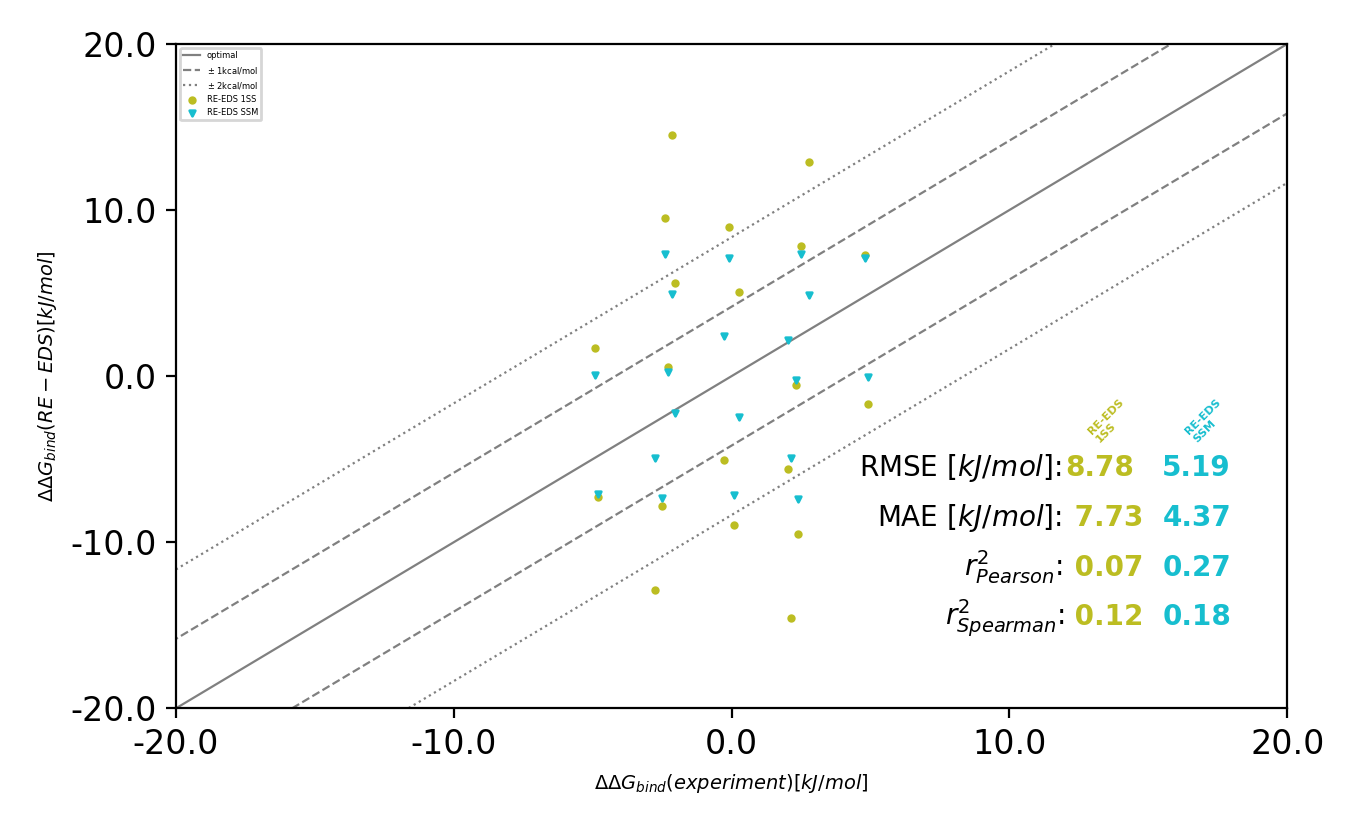
\includegraphics[width=0.8\textwidth]{fig/results/ringOpening/paramOptimization/RingClosure_system_Eoff_final_results.png}
\caption{Comparison of the relative energy offsets $\Delta \Delta E^R_{ji}$ in water and complex with the experimental relative binding free energies $\Delta \Delta G^\text{bind}_{ji}$. The energy offsets were estimated from RE-EDS simulations using the 1SS (green) or SSM (blue) approach to select the starting configurations of the replicas.} \label{SIfig:Eoff_experiment_corr_RingOpening}
\end{figure}

\newpage
\section{Optimization of the $s$-Distribution and the energy offsets}
\begin{figure}[h]
\centering
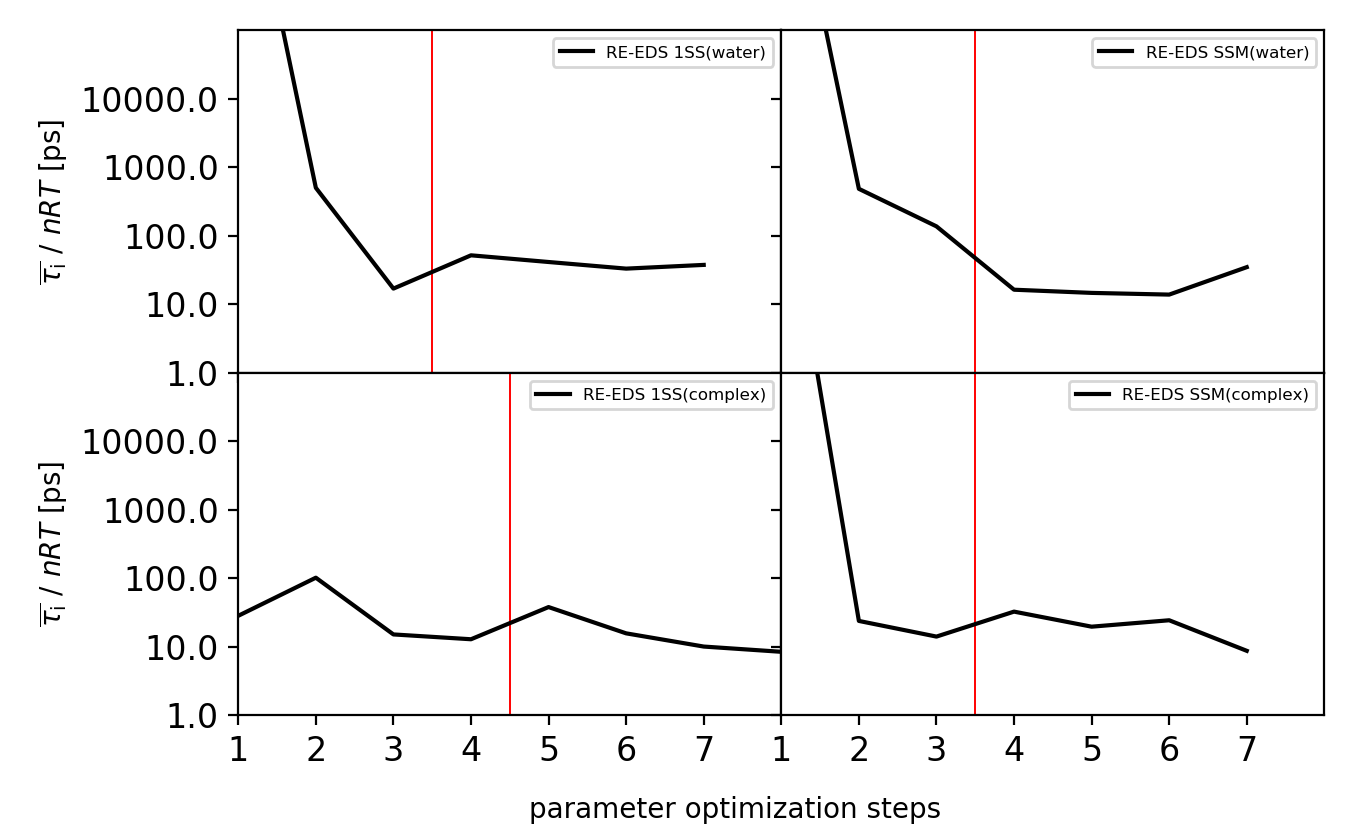
\includegraphics[width=\linewidth]{fig/results/ringOpening/paramOptimization/RingOpening_optimization_RTstat.png}
\caption{Average round-trip time as a function of the optimization steps $i$ ($\overline{\tau}_i$) on a logarithmic scale. The red line indicates the switch from $s$-optimization to energy offset rebalancing.}
\label{SIfig:CHK1_RingOpening_soptimization_efficiency}
\end{figure}

\begin{figure}[H]
\centering
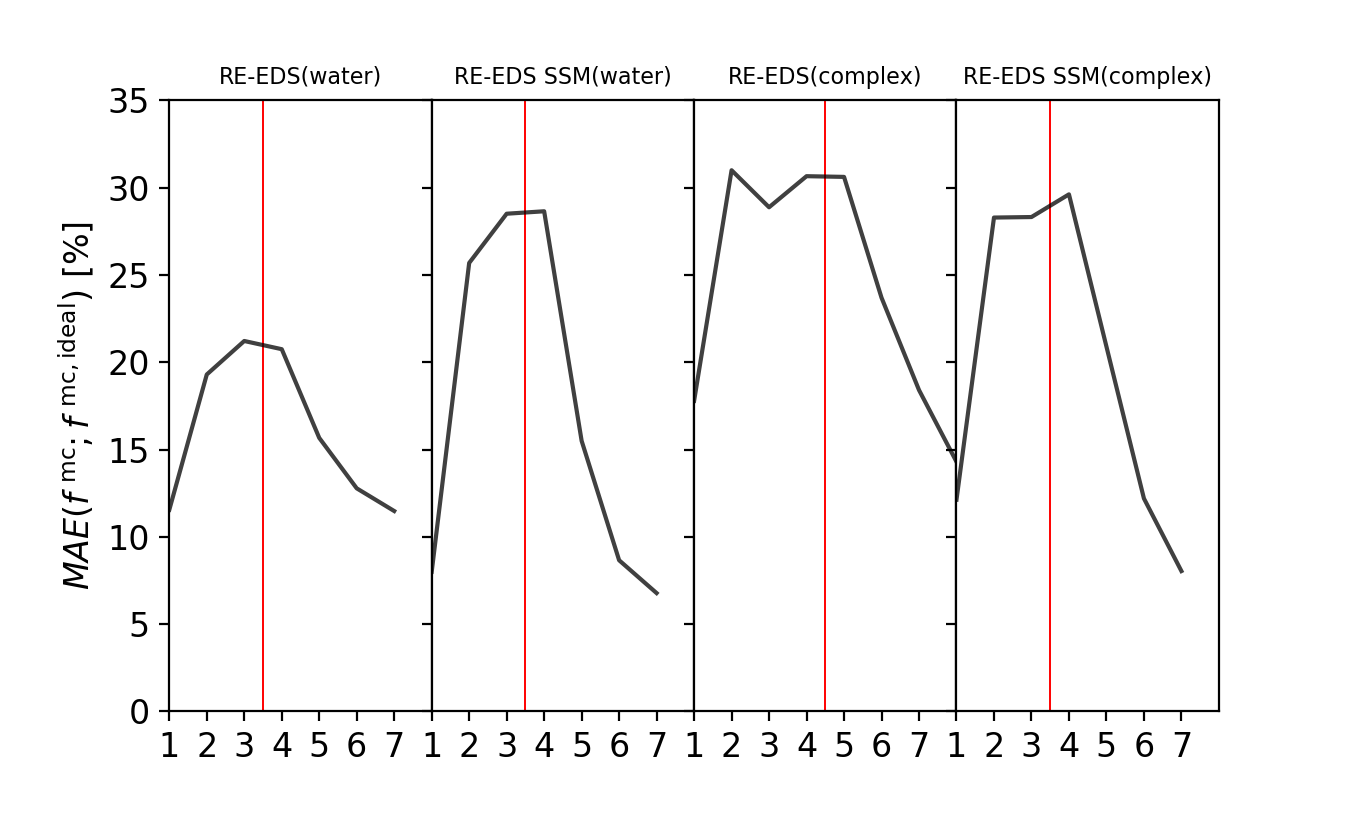
\includegraphics[width=\linewidth]{fig/results/ringOpening/paramOptimization/RingOpening_optimization_fractOptSampMAE.png}
\caption{Mean absolute deviation (MAE, in percentage) of the observed state sampling $f_i^{\text{mc}}$ from the ideal equal distribution $f_i^{\text{mc,ideal}}$ during the short optimization simulations. The red line indicates the switch from $s$-optimization to energy offset rebalancing.}
\label{SIfig:CHK1_RingOpening_optimization_fractOptSampMAE}
\end{figure}

\newpage
\section{Free-Energy Calculation}
\begin{table}[H]
\caption{Free-energy differences in water and in complex calculated from the production run of 3.5~ns of length with the RE-EDS 1SS and RE-EDS SSM approaches.}
\begin{center}
\begin{tabular}{ c c |c c |c c}
  \multicolumn{2}{c|}{Ligand} & \multicolumn{2}{c|}{RE-EDS 1SS} &\multicolumn{2}{c}{RE-EDS SSM}\\ 
  J & I  & water [kJ~mol$^{-1}$] & complex [kJ~mol$^{-1}$]  & water [kJ~mol$^{-1}$] & complex [kJ~mol$^{-1}$] \\
  \hline
        L17 &         L1 &       11.9 $\pm$ 0.0&       12.4 $\pm$ 0.5&   17.0 $\pm$ 0.8&   9.4 $\pm$ 1.9\\
        L19 &         L1 &        2.7 $\pm$ 0.0&        3.1 $\pm$ 0.0&    5.7 $\pm$ 1.0&   8.0 $\pm$ 0.0\\
        L20 &         L1 &      -47.8 $\pm$ 0.0&      -47.7 $\pm$ 0.0& -47.6 $\pm$ 0.9&  -48.1 $\pm$ 0.0\\
        L21 &         L1 &      -61.7 $\pm$ 0.06&     -61.7 $\pm$ 0.0& -63.1 $\pm$ 0.8&  -64.8 $\pm$ 0.0\\
        L19 &         L17 &      -9.2 $\pm$ 0.0&       -9.3 $\pm$ 0.5& -11.3 $\pm$ 0.6&   -1.4 $\pm$ 1.9\\
        L20 &         L17 &     -59.6 $\pm$ 0.0&      -60.1 $\pm$ 0.5& -64.5 $\pm$ 0.1&  -57.6 $\pm$ 1.9\\
        L21 &         L17 &     -73.6 $\pm$ 0.0&      -74.1 $\pm$ 0.5& -80.1 $\pm$ 0.1&  -74.3 $\pm$ 1.9\\
        L20 &         L19 &     -50.5 $\pm$ 0.0&      -50.7 $\pm$ 0.0& -53.2 $\pm$ 0.6&  -56.2 $\pm$ 0.0\\
        L21 &         L19 &     -64.4 $\pm$ 0.0&      -64.7 $\pm$ 0.0& -68.8 $\pm$ 0.6&  -72.9 $\pm$ 0.0\\
        L21 &         L20 &     -13.9 $\pm$ 0.0&      -14.0 $\pm$ 0.0& -15.5 $\pm$ 0.18& -16.7 $\pm$ 0.0 \\
\end{tabular}
\end{center}
\label{SItab: RE-EDS_FE_RingCycleOpening_dFs}
\end{table}


\begin{figure}[H]
\centering
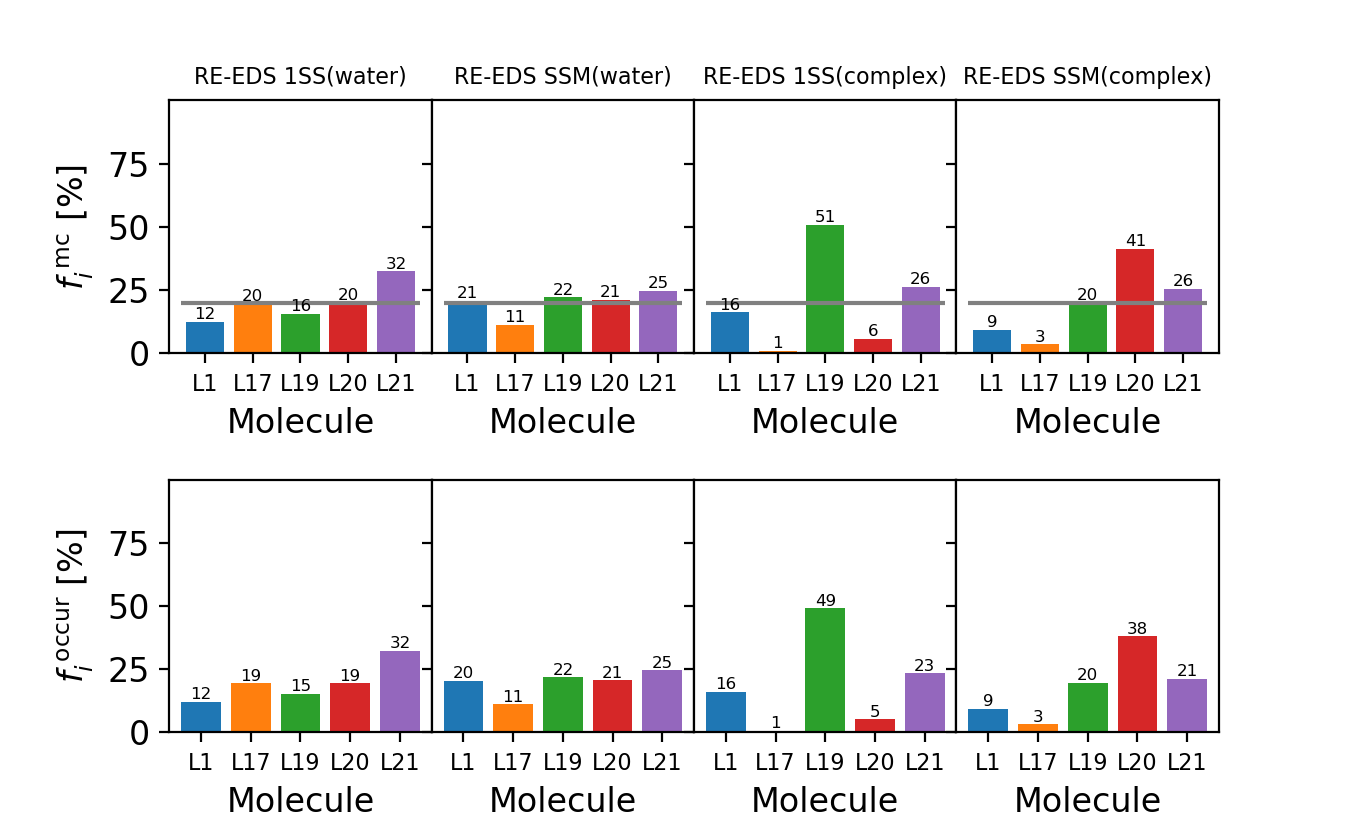
\includegraphics[width=\linewidth]{fig/results/ringOpening/FE/Reeds_RingOpening_production_sampling_s1.png}
\caption{Sampling of the end states in the final production run at replica $s=1.0$. Sampling was assessed by monitoring the maximally contributing end state (top panels) and by counting all end states a potential energy below $T_{i}^{phys}$ (see Table \ref{SItab:RingCycleOpenin_PotentialTresholds}) (bottom panels). Ideally, the sampling fraction as maximally contributing end state should be 1/$N$ (Eq. (8) in the main text) for all end states, indicated as a black horizontal line.}
\label{SIfig:CHK1_RingOpening_soptimization_final_Sampling_s1}
\end{figure}


\begin{figure}[H]
\centering
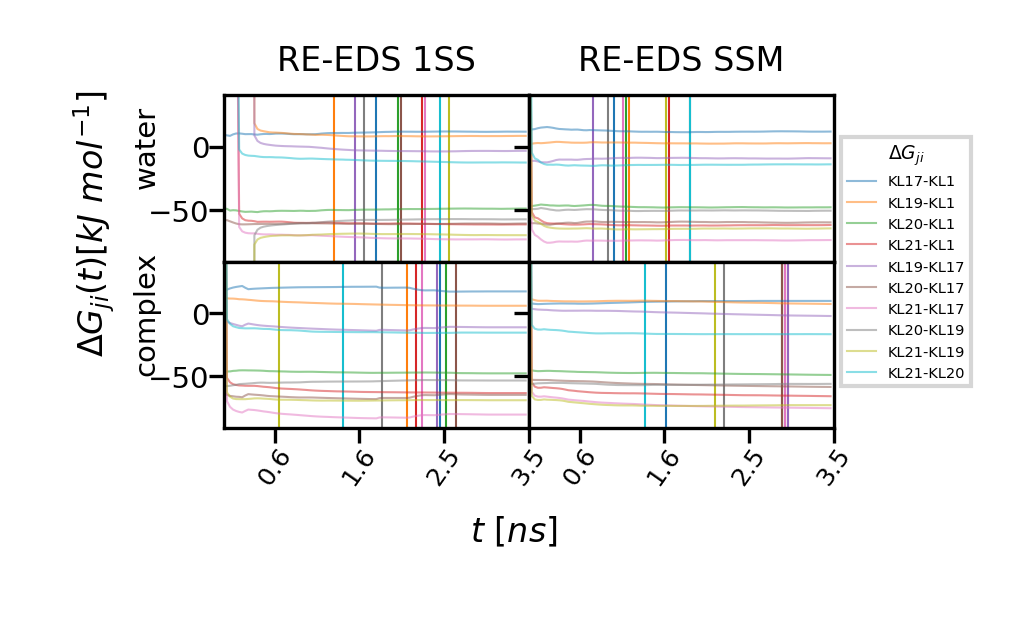
\includegraphics[width=\linewidth]{fig/results/ringOpening/FE/dF_RingOpening_Convergence.png}
\caption{Convergence analysis of the RE-EDS production runs (total 3.5~ns): The free-energy results are plotted as a function of the simulation time. The vertical lines indicate when a particular $\Delta G_{ji}$ value was found to be converged (deviation below 1~kJ~mol$^{-1}$).}
\label{SIfig:CHK1_RingOpening_dF_convergence}
\end{figure}


\clearpage
\newpage

%================================================================================
\section{Conclusion}
%================================================================================

This study reports the recent developments for the multistate free-energy method RE-EDS, which omits the definition of alchemical transition paths. The automatic workflow for RE-EDS was improved in robustness, and was applied to estimate the relative binding free energies of five CHK1 inhibitors containing typical core-hopping transformations. This system was investigated previously with FEP+ and QligFEP, allowing for a direct comparison of RE-EDS with state-of-the-art pairwise free-energy methods.
Using different starting configurations representing all end states (SSM approach) in the parameter optimization of the RE-EDS workflow improved the sampling, convergence, and the accuracy of the resulting free-energy differences. The performance of RE-EDS SSM was found to be comparable with FEP+ and QligFEP, and shows that RE-EDS with a ``dual topology" approach can be readily applied to challenging ligand transformations like ring size change, ring opening/closing, and ring extension.

In terms of computational efficiency, the total production run time with RE-EDS ($4$~ns per replica) was about half of that reported for FEP+ with this system. For RE-EDS, the simulation time could have been reduced further as the free-energy differences were found to be converged already after about $1$~ns. As multiple ligands are simulated simultaneously in a single RE-EDS simulation, this sampling enhancement will increase with increasing number of ligands. 
However, the pre-processing phase in the RE-EDS workflow currently uses a relatively large amount of simulation time. Making these steps more efficient will be addressed in future work.

The Python code for the RE-EDS workflow is provided on Github \\https://github.com/rinikerlab/reeds and can be used with the current version of GROMOS, freely available from http://www.gromos.net.

\clearpage
\pagebreak

%\bibliography{4_chapter_2/ref/ref.bib}


\end{document}

